%%%%%%%%%%%%%%%%%%%%%%%%%%%%%%%%%%%%%%%%%%%%%%%%%%%%%%%%%%%%%%%%%%%%%%%%%%%%%%%%%%%%%%%%%
% Khóa luận tốt nghiệp/Tiểu luận 
% LaTeX Template
% Phiên bản 1.0 (tạo ra ngày 05/10/2022)
%
% Template này có thể được download tại:
% https://github.com/cpc1996/HUS-Dissertation-Template
%
% Phiên bản 1.0 được chỉnh sửa bởi:
% Công Phương Cao (congphuongcao_t59@hus.edu.vn)
% Nguyễn Cảnh Việt (vietncp@gmail.com)
% Nguyễn Tiến Cường (ngtiencuong@gmail.com)
%
% Template được tham khảo từ một phiên bản template của:
% Steve Gunn (http://users.ecs.soton.ac.uk/srg/softwaretools/document/templates/)
% Sunil Patel (http://www.sunilpatel.co.uk/thesis-template/)
%
%%%%%%%%%%%%%%%%%%%%%%%%%%%%%%%%%%%%%%%%%%%%%%%%%%%%%%%%%%%%%%%%%%%%%%%%%%%%%%%%%%%%%%%%%


%----------------------------------------------------------------------------------------
%	(KHÔNG CHỈNH SỬA PHẦN NÀY)
%
%	PHẦN 1: CÁC PACKAGE CƠ BẢN VÀ CÁC TÙY CHỈNH VĂN BẢN
%----------------------------------------------------------------------------------------

\documentclass[
12pt,
oneside,
english,
doublespacing,
nolistspacing,
liststotoc,
parskip,
headsepline,
chapterinoneline,
]{MastersDoctoralThesis}

% \usepackage[utf8]{inputenc} 
\usepackage[utf8]{vietnam} 
%\usepackage[T1]{fontenc}

\usepackage{mathptmx}
\usepackage{amsmath}
\allowdisplaybreaks

%https://www.overleaf.com/learn/latex/Biblatex_citation_styles
%\usepackage[backend=bibtex,style=authoryear,natbib=true]{biblatex}
\usepackage[backend=bibtex,style=numeric,citestyle=ieee,natbib=true]{biblatex}

\addbibresource{main.bib}

\usepackage[autostyle=true]{csquotes}


%----------------------------------------------------------------------------------------
%	PHẦN 2: CÁC PACKAGE BỔ TRỢ THÊM VÀO TRONG QUÁ TRÌNH BIÊN SOẠN
%----------------------------------------------------------------------------------------

\usepackage{multirow}
\usepackage{subfigure}
\usepackage[fontsize=13pt]{scrextend}

%https://www.sascha-frank.com/latex-font-size.html
%https://tex.stackexchange.com/questions/103286/how-to-change-section-subsection-font-size
\usepackage{titlesec}

\titleformat{\section}
{\normalfont\fontsize{13}{13}\bfseries}{\thesection}{1em}{}

\titleformat{\subsection}
{\normalfont\fontsize{13}{13}\bfseries\itshape}{\thesubsection}{1em}{}

\usepackage{listings} 		% Liệt kê/trích dẫn code

%https://tex.stackexchange.com/questions/351961/how-to-indent-code-in-beginverbatim
\usepackage{fancyvrb} 		% Fancy Verbatim
\fvset{tabsize=4,vspace=0pt,fontsize=\footnotesize}

\usepackage{longtable} 		% Bảng dài - Long table

\usepackage[figuresright]{rotating} % Bảng ngang - Sideways table
\usepackage{tabularx}

\usepackage{fontawesome5} 	% Các biểu tượng, ký hiệu đặc biệt

\usepackage{tikz} 			% Vẽ hình
\usetikzlibrary{calc}


%----------------------------------------------------------------------------------------
%	(KHÔNG CHỈNH SỬA PHẦN NÀY)
%
%	PHẦN 3: CÁC TÙY CHỈNH LIỆT KÊ SOURCE CODE 
%----------------------------------------------------------------------------------------

%https://tex.stackexchange.com/questions/33039/using-ttfamily-with-bfseries-or-how-to-enable-bold-in-fixed-width-font
\renewcommand{\ttdefault}{pcr}
\newenvironment{pcr}{\fontfamily{pcr}\selectfont}

\definecolor{backcolor}{HTML}{f5fffc}
\definecolor{darkpink}{rgb}{0.75,0.25,0.5}
\definecolor{cadetblue}{rgb}{.6,.8,.8}

\lstset{
	tabsize			= 4,
	breaklines		= true,
	basicstyle		= \ttfamily\color{black}\bfseries\scriptsize,
	identifierstyle	= \ttfamily\color{black},
	keywordstyle	= \ttfamily\color{blue}\bfseries,  
	stringstyle		= \ttfamily\color{Red},
	commentstyle	= \itshape\color{cyan},
	%===================================================================================
	frame			= l,
	numbers			= left,
	stepnumber		= 1, 
	upquote			= true,
	numberstyle		= \tiny\color{Gray},
	backgroundcolor	= \color{backcolor},
	rulecolor		= \color{lightgray},
	rulesepcolor	= \color{lightgray},
	showstringspaces=false
	keepspaces		= true, 
	belowcaptionskip= 1\baselineskip,
	xleftmargin		= \parindent,
	%	escapeinside	= {@}{@},
	numbersep		= 7pt
}

\lstdefinestyle{codeC} {
	%https://www.pvv.ntnu.no/~berland/latex/docs/listings.pdf
	%https://www.overleaf.com/learn/latex/Using_colours_in_LaTeX
	language		= [ISO]C++, 
	basicstyle		= \linespread{1.0}\ttfamily\color{black}\bfseries\scriptsize,
	identifierstyle	= \ttfamily\color{black},
	keywordstyle	= \ttfamily\color{blue}\bfseries,  
	stringstyle		= \ttfamily\color{Red},
	commentstyle	= \itshape\color{cyan}, 
	morekeywords	= {FILE},
	%	emphstyle		= \ttfamily\color{red}\bfseries,
	%	emph			= { auto,break,case,char,const,continue,default,do,double,else,enum,extern,float,for,goto,if,int,long,register,return,short,signed,sizeof,static,struct,switch,typedef,union,unsigned,void,volatile,while,FILE},
	%https://tex.stackexchange.com/questions/283170/using-different-colors-for-different-keywords-in-lstlisting
	classoffset		= 1, % starting new class
	otherkeywords	= {\#include},
	morekeywords	= {\#include},
	keywordstyle	= \ttfamily\color{Green}\bfseries,
	morecomment		= [s][\bfseries\color{Orange}]{<a}{>},% a b d e f i l m n q r s t u v
	morecomment		= [s][\bfseries\color{Orange}]{<b}{>},
	morecomment		= [s][\bfseries\color{Orange}]{<d}{>},
	morecomment		= [s][\bfseries\color{Orange}]{<e}{>},
	morecomment		= [s][\bfseries\color{Orange}]{<f}{>},
	morecomment		= [s][\bfseries\color{Orange}]{<i}{>},
	morecomment		= [s][\bfseries\color{Orange}]{<l}{>},
	morecomment		= [s][\bfseries\color{Orange}]{<m}{>},
	morecomment		= [s][\bfseries\color{Orange}]{<n}{>},
	morecomment		= [s][\bfseries\color{Orange}]{<q}{>},
	morecomment		= [s][\bfseries\color{Orange}]{<r}{>},
	morecomment		= [s][\bfseries\color{Orange}]{<s}{>},
	morecomment		= [s][\bfseries\color{Orange}]{<t}{>},
	morecomment		= [s][\bfseries\color{Orange}]{<u}{>},
	morecomment		= [s][\bfseries\color{Orange}]{<v}{>},
	morecomment		= [l][\bfseries\color{Green}]{\#define},
	classoffset		= 0,
}

\lstdefinestyle{plaintext} {
	%https://www.pvv.ntnu.no/~berland/latex/docs/listings.pdf
	%https://www.overleaf.com/learn/latex/Using_colours_in_LaTeX
	language		= bash, 
	basicstyle		= \linespread{1.0}\ttfamily\color{black}\bfseries\scriptsize,
	identifierstyle	= \ttfamily\color{black},
	keywordstyle	= \ttfamily\color{black}\bfseries,  
	stringstyle		= \ttfamily\color{black},
	commentstyle	= \itshape\color{gray}, 
	%	showspaces		= true,
	%	showstringspaces= true,
	showtabs		= true,
	tab				= \textcolor{lightgray}{$\to$},
%	literate=*
%	{0}{{{\color{darkpink}0}}}{1}
}

\lstdefinestyle{codeMatlab} {
	language		= Matlab,
	basicstyle		= \linespread{1.0}\ttfamily\color{black}\bfseries\scriptsize,
	identifierstyle	= \ttfamily\color{black},
	keywordstyle	= \ttfamily\color{blue}\bfseries,  
	stringstyle		= \ttfamily\color{magenta},
	commentstyle	= \itshape\color{LimeGreen},
	morecomment		= [l][\bfseries\color{red}]{\%\%},
	morekeywords	= {syms,switch,case,otherwise,ones,class,inline,vectorize,factorial,xlim,ylim,ezplot,pie,ezmesh,ezsurf,ezcontour,ezplot3,solve,double,subs,fsolve,fminsearch,compose,jacobian,int,dblquad,triplequad,limit,finverse,simplify,taylor,symsum,evalin,symengine,matlabFunction,poly2sym,lsqcurvefit,ppval,dsolve},
	literate		=*,
	literate		=*
	{^}{\textasciicircum}{1}
}

\lstdefinestyle{codePython} {
	language		= Python,
	basicstyle		= \linespread{1.0}\ttfamily\color{black}\bfseries\scriptsize,
	identifierstyle	= \ttfamily\color{black},
	keywordstyle	= \ttfamily\color{blue}\bfseries,  
	stringstyle		= \ttfamily\color{LimeGreen},
	commentstyle	= \itshape\color{cadetblue},
	morekeywords	= {self},
	emph			={MyClass,__init__},
	emphstyle		=\ttb\color{red},
	literate		=*,
	literate		=*
	{^}{\textasciicircum}{1}
}

%https://www.alanshawn.com/tech/2019/09/01/emulate-terminal.html
\definecolor{tergreen}{rgb}{0,0.6,0}
\definecolor{tergray}{rgb}{0.5,0.5,0.5}
\definecolor{termauve}{rgb}{0.58,0,0.82}
\definecolor{terminalbgcolor}{HTML}{330033}
\definecolor{terminalrulecolor}{HTML}{000099}
\lstdefinestyle{console} {
	backgroundcolor	= \color{terminalbgcolor},
	basicstyle		= \linespread{1.0}\ttfamily\color{white}\bfseries\scriptsize,
	identifierstyle	= \ttfamily\color{white}\bfseries\scriptsize,
	breakatwhitespace=false,
	breaklines		= true,
	captionpos		= b,
	commentstyle	= \color{tergreen},
	deletekeywords	= {...},
	escapeinside	= {\%*}{*)},
	extendedchars	= true,
	frame			= single,
	keepspaces		= true,
	keywordstyle	= \color{blue},
	language		= {},
	morekeywords	= {*,...},
	numbers			= none,
	numbersep		= 5pt,
	framerule		= 2pt,
	numberstyle		= \color{tergray}\tiny\selectfont,
	rulecolor		= \color{terminalrulecolor},
	showspaces		= false,
	showstringspaces= false,
	showtabs		= false,
	stepnumber		= 2,
	stringstyle		= \color{termauve},
	tabsize			= 2,
	literate		=*
}


%----------------------------------------------------------------------------------------
%	(KHÔNG CHỈNH SỬA PHẦN NÀY)
%
%	PHẦN 4: CÁC TÙY CHỈNH KHỔ GIẤY VÀ CĂN LỀ
%----------------------------------------------------------------------------------------

\geometry{
	paper=a4paper,
	inner=3cm,
	outer=2cm,
	bindingoffset=0cm,
	top=0.6cm,
	bottom=2.0cm,
}


%----------------------------------------------------------------------------------------
%	PHẦN 5: THÔNG TIN VỀ Khóa luận tốt nghiệp/Tiểu luận (THESIS INFORMATION)
%----------------------------------------------------------------------------------------

\author{Tên sinh viên thực hiện} 			% Ví dụ: "Nguyễn Thị Thu Thảo"
\thesistitle{Tên của Khóa luận tốt nghiệp/Tiểu luận} % Ví dụ: "Nghiên cứu chế tạo và tính chất quang học của vật liệu nano LaF3:Sm3+"

\supervisor {Tên giảng viên hướng dẫn 1} 	% Ví dụ: "PGS. TS. Nguyễn Ngọc Long"
\supervisorr{Tên giảng viên hướng dẫn 2} 	% Tên này nếu không có thì để trống!

\field{Tên ngành đào tạo} 					% Ví dụ: "Ngành Vật lý", "Ngành Hóa học", v.v.
\program{Tên chương trình đào tạo} 			% Ví dụ: "Chương trình đào tạo chuẩn", "Chương trình đào tạo cử nhân tài năng", v.v.
\doctype{Khóa luận tốt nghiệp đại học hệ chính quy} % Điền vào đây: "Khóa luận tốt nghiệp đại học hệ chính quy" hoặc "Tiểu luận"

\university{\href{http://hus.vnu.edu.vn}{Trường Đại học Khoa học Tự nhiên}}
\department{\href{http://hus.vnu.edu.vn/gioi-thieu/co-cau-to-chuc/khoa-truc-thuoc/khoa-vat-ly.html}{Khoa Vật lý}}

\AtBeginDocument{
	\hypersetup{pdftitle=\ttitle}
	\hypersetup{pdfauthor=\authorname}
}


\begin{document}

\lstset{style=codeC}	% Thiết lập ngôn ngữ C/C++ là ngôn ngữ mặc định cho phần liệt kê souce code của cả bài

\frontmatter 			% Sử dụng hệ thống đánh số La Mã (i, ii, iii, iv...) cho những trang trước phần mục lục

\pagestyle{plain} 


%----------------------------------------------------------------------------------------
%	(KHÔNG CHỈNH SỬA PHẦN NÀY)
%
%	Phần 6: TRANG TIÊU ĐỀ/TRANG BÌA (TITLE PAGE)
%----------------------------------------------------------------------------------------

% TRANG BÌA CHÍNH:
%----------------------------------------------------------------------------------------
%	(KHÔNG CHỈNH SỬA PHẦN NÀY)
%
%	Phần 6: TRANG TIÊU ĐỀ/TRANG BÌA (TITLE PAGE)
%----------------------------------------------------------------------------------------

% TRANG BÌA CHÍNH:
\begin{titlepage}
	\begin{tikzpicture}[overlay,remember picture]
		\draw [line width=3pt]
		($ (current page.north west) + (2.0cm,-2.0cm) $)
		rectangle
		($ (current page.south east) + (-1.5cm,1.8cm) $);
		\draw [line width=1pt]
		($ (current page.north west) + (2.15cm,-2.15cm) $)
		rectangle
		($ (current page.south east) + (-1.65cm,1.95cm) $); 
	\end{tikzpicture}
	\begin{center}
		
		\vspace{-.04\textheight}
		\noindent%\scshape
		\large \, \href{https://www.vnu.edu.vn/home/}{ĐẠI HỌC QUỐC GIA HÀ NỘI}\\
		\vspace{-0.25cm}{\large \MakeUppercase \univname}\\
		\vspace{-0.25cm}{\large \bfseries \MakeUppercase \deptname}\\[0.5cm]
		
\includegraphics{Logo/Logo_HUS_notext_nocolor}
		
		\vspace{1.0cm}
		
		{\large \MakeUppercase \authorname}
		
		\vspace{2.5cm}
		
		{\Large \bfseries \MakeUppercase\ttitle\par}
		
		\vspace{2.5cm}
		
		{\normalsize \docname\\ \fieldname\\ (\progname)\\}
		
		\vfill
		
		\textbf{Hà Nội - \the\year{}}
	\end{center}
\end{titlepage}



% TRANG BÌA PHỤ:
%----------------------------------------------------------------------------------------
%	(KHÔNG CHỈNH SỬA PHẦN NÀY)
%
%	Phần 6: TRANG TIÊU ĐỀ/TRANG BÌA (TITLE PAGE)
%----------------------------------------------------------------------------------------

% TRANG BÌA PHỤ:
\begin{titlepage}
	\begin{tikzpicture}[overlay,remember picture]
		\draw [line width=3pt]
		($ (current page.north west) + (2.0cm,-2.0cm) $)
		rectangle
		($ (current page.south east) + (-1.5cm,1.8cm) $);
		\draw [line width=1pt]
		($ (current page.north west) + (2.15cm,-2.15cm) $)
		rectangle
		($ (current page.south east) + (-1.65cm,1.95cm) $); 
	\end{tikzpicture}
	\begin{center}
		
		\vspace{-.04\textheight}
		\noindent\scshape
		\large \, \href{https://www.vnu.edu.vn/home/}{ĐẠI HỌC QUỐC GIA HÀ NỘI}\\
		\vspace{-0.25cm}{\large \MakeUppercase \univname}\\
		\vspace{-0.25cm}{\large \bfseries \MakeUppercase \deptname}\\[0.5cm]
		
\includegraphics{Logo/Logo_HUS_notext}
		
		\vspace{1.0cm}
		
		{\large \MakeUppercase \authorname}
		
		\vspace{2.5cm}
		
		{\Large \bfseries \MakeUppercase\ttitle\par}
		
		\vspace{2.5cm}
		
		{\normalsize \docname\\ \fieldname\\ (\progname)\\}
		
		\vspace{2.5cm}
		
		\begin{minipage}[t]{0.49\textwidth}
			\begin{flushright} \large \bfseries
				Giảng viên hướng dẫn:\;
			\end{flushright}
		\end{minipage}
		\begin{minipage}[t]{0.5\textwidth}
			\begin{flushleft} \large \bfseries
				\supname\\
				\supnamee
			\end{flushleft}
		\end{minipage}
		
		\vfill
		
		\textbf{Hà Nội - \the\year{}}
	\end{center}
\end{titlepage}




%----------------------------------------------------------------------------------------
%	Phần 7: DANH NGÔN (QUOTES)
%----------------------------------------------------------------------------------------

\vspace*{0.2\textheight}

\noindent\enquote{\itshape 
	Cái tôi và sự hiểu biết tỷ lệ nghịch với nhau. Hiểu biết càng nhiều cái tôi càng bé. Hiểu biết càng ít, cái tôi càng to.
}\bigbreak

\hfill Albert Einstein


%----------------------------------------------------------------------------------------
%	Phần 8: LỜI CẢM ƠN (ACKNOWLEDGEMENTS)
%----------------------------------------------------------------------------------------

\begin{acknowledgements}
	\addchaptertocentry{\acknowledgementname}
	\thispagestyle{empty}
	Sự ghi nhận và lời cảm ơn đối đối với những người liên quan, đừng quên cảm ơn giảng viên hướng dẫn của bạn\ldots
\end{acknowledgements}


%----------------------------------------------------------------------------------------
%	(KHÔNG CHỈNH SỬA PHẦN NÀY)
%
%	Phần 9: MỤC LỤC (LIST OF CONTENTS/FIGURES/TABLES PAGES)
%----------------------------------------------------------------------------------------

\begin{spacing}{1.15}
	\tableofcontents 	% In ra mục lục chính
\end{spacing}

\begin{spacing}{1.15}
	\listoffigures 		% In ra danh sách hình vẽ
\end{spacing}

\begin{spacing}{1.15}
	\listoftables		% In ra danh sách bảng
\end{spacing}


%----------------------------------------------------------------------------------------
%	Phần 10: DANH SÁCH TÊN VIẾT TẮT (ABBREVIATIONS)
%----------------------------------------------------------------------------------------

\begin{abbreviations}{ll} % Thêm danh sách tên viết tắt (dưới dạng một bảng có 2 cột)

\textbf{TVT} & \textbf{T}ên \textbf{V}iết \textbf{T}ắt\\
\textbf{ĐTĐ} & \textbf{Đ}ặt (nó) \textbf{T}ại \textbf{Đ}ây\\

\end{abbreviations}


%----------------------------------------------------------------------------------------
%	Phần 11: CÁC HẰNG SỐ VẬT LÝ/THÔNG SỐ KĨ THUẬT (PHYSICAL CONSTANTS/OTHER DEFINITIONS)
%----------------------------------------------------------------------------------------

\begin{constants}{lr@{${}={}$}l} % Thêm danh sách các hằng số (dưới dạng một bảng có 3 cột)

%	Lệnh \SI{}{} được cung cấp bởi gói siunitx, hãy đọc tài liệu hướng dẫn để biết cách sử dụng nó

%	Tên hằng số 	 & $Biểu tượng$	& $Hằng số$ cùng với đơn vị\\
	Vận tốc ánh sáng & $c_{0}$		& \SI{2.99792458e8}{\meter\per\second} (chính xác)\\

\end{constants}


%----------------------------------------------------------------------------------------
%	Phần 12: DANH SÁCH KÝ HIỆU (SYMBOLS)
%----------------------------------------------------------------------------------------

\begin{symbols}{lll} % Thêm danh sách các ký hiệu (dưới dạng một bảng có 3 cột)

%   Ký hiệu	& Ý nghĩa		& Đơn vị \\
	$a$		& khoảng cách	& \si{\meter} \\
	$P$		& công suất		& \si{\watt} (\si{\joule\per\second}) \\

	\addlinespace % Khoảng cách để phân biệt giữa ký hiệu Latin với ký hiệu La Mã

	$\omega$ & tần số góc	& \si{\radian} \\

\end{symbols}


%----------------------------------------------------------------------------------------
%	(KHÔNG CHỈNH SỬA PHẦN NÀY)
%
%	Phần 13: LỜI ĐỀ TẶNG (DEDICATION)
%----------------------------------------------------------------------------------------

%\dedicatory{Dành tặng/Dành cho/Gửi tới\ldots} 


%----------------------------------------------------------------------------------------
%	Phần 14: NỘI DUNG/CÁC CHƯƠNG Khóa luận tốt nghiệp/Tiểu luận (THESIS CONTENT - CHAPTERS)
%----------------------------------------------------------------------------------------

\mainmatter % Bắt đầu đánh số trang (1,2,3...)

\pagestyle{plain}

% Hãy thêm những chương (chapter) của khóa luận/tiểu luận vào thư mục Chapters
% Hãy bỏ chú thích những dòng nếu bạn đã bổ sung những chương vào

% MỞ ĐẦU (LỜI MỞ ĐẦU - Chương 0)

\chapter*{MỞ ĐẦU} % Tên của chương
\addcontentsline{toc}{chapter}{MỞ ĐẦU} % Thêm tên chương vào mục lục

\label{Chapter0} % Để trích dẫn chương này ở chỗ nào đó trong bài, hãy sử dụng lệnh \ref{Chapter0} 

%----------------------------------------------------------------------------------------

Xử lý ngôn ngữ tự nhiên (NLP) là một lĩnh vực học máy đang ngày càng phổ biến trong các lĩnh vực như AI, Robotics, Data science, ... và ngày càng có tầm ảnh hưởng lớn hơn trong cuộc cách mạng 4.0 của thế giới.

Bài nghiên cứu này trình bày về xử lý ngôn ngữ tự nhiên và các thuật toán cho đề tài "Nghiên cứu phân tích văn bản trong học máy". Nội dung của bài nghiên cứu này gồm 4 chương và 1 phụ lục:

\begin{enumerate}
	\item \textbf{Chương \ref{Chapter1}: Xử lý ngôn ngữ tự nhiên - Natural language proccessing}\\
	Giới thiệu về NLP và các framework được sử dụng rộng rãi trong lĩnh vực này
	\item \textbf{Chương \ref{Chapter2}: Feature Engineering và các model xử lý dữ liệu dạng văn bản}\\
	Giới thiệu về Feature Engineering (Kĩ thuật phổ biến trong các bài toán về học máy) và các model đã và đang được áp dụng vào NLP
	\item \textbf{Chương \ref{Chapter3}: Topic Modeling}
	Một bài toán đặc trưng của xử lý dữ liệu dạng văn bản \\
	Các thuật toán như \textbf{LSA và LDA}
	\item \textbf{Chương \ref{Chapter4}: Các model nâng cao trong xử lý dữ liệu dạng văn bản}\\
	Các model giải quyết các bài toán phức tạp hơn của việc xử lý ngôn ngữ và là sự cải tiến của các model được giới thiệu ở Chương \ref{Chapter2}
	\item \textbf{Phụ lục \ref{AppendixB}: Liệt kê source code} 
\end{enumerate}


% Chương 1

\chapter{MỞ ĐẦU - GIỚI THIỆU CHUNG} % Tên của chương

\label{Chapter1} % Để trích dẫn chương này ở chỗ nào đó trong bài, hãy sử dụng lệnh \ref{Chapter1} 

%----------------------------------------------------------------------------------------

% Định nghĩa một số lệnh cần thiết để điều chỉnh định dạng cho một số nội dung nhất định trong bài
\newcommand{\keyword}[1]{\textbf{#1}}
\newcommand{\tabhead}[1]{\textbf{#1}}
\newcommand{\code}[1]{\texttt{#1}}
\newcommand{\file}[1]{\texttt{\bfseries#1}}
\newcommand{\option}[1]{\texttt{\itshape#1}}

%----------------------------------------------------------------------------------------

\section{Lời mở đầu}

Chào mừng bạn đến với template \LaTeX{} khóa luận tốt nghiệp/tiểu luận của Bộ môn Tin học Vật lý. Đây là một template đẹp và dễ sử dụng cho việc biên soạn khóa luận tốt nghiệp/tiểu luận sử dụng hệ thống gõ \LaTeX{}.

Nếu bạn đang hoặc sẽ biên soạn khóa luận tốt nghiệp/tiểu luận và chủ đề liên quan đến kĩ thuật hoặc toán học thì việc biên soạn trên \LaTeX{} là rất đáng cân nhắc vì đây là cách giúp bạn có thể ngồi xuống và tập trung vào nội dung viết cốt lõi mà không cần lo lắng về mặt định dạng (format) cũng như lãng phí thời gian vào việc tinh chỉnh phần mềm soạn thảo văn bản.

\LaTeX{} có thể dễ dàng biên soạn các tài liệu một cách chuyên nghiệp mà lên tới hàng trăm hoặc hàng nghìn trang. Với câu lệnh đơn giản, nó tự động sắp đặt mục lục, lề, tiêu đề/chân trang, và giữ cho định dạng thống nhất và đẹp đẽ. Một trong những thế mạnh chính của \LaTeX{} là việc gõ các công thức toán học, thậm chí các công thức \emph{rất phức tạp}. Ngay cả khi những phương trình này là những vấn đề phức tạp và khó khăn nhất mà chỉ có thể được giải được bằng siêu máy tính, bạn có thể yên tâm là ít nhất \LaTeX{} sẽ làm cho chúng trông \emph{lộng lẫy}.


%----------------------------------------------------------------------------------------

\section{Học \LaTeX{}}

\LaTeX{} không phải một chương trình \textsc{wysiwyg} (What You See is What You Get, tạm dịch: \textit{Giao diện tương tác tức thời - mắt thấy tay làm}), không giống các trình soạn thảo văn bản như Microsoft Word hoặc Pages của Apple. Một văn bản được viết cho \LaTeX{} chỉ đơn thuần là một file (tập tin) văn bản đơn giản \emph{không có định dạng}. Bạn nói với \LaTeX{} cách bạn muốn văn bản định dạng bằng cách viết những dòng lệnh đơn giản trong văn bản, ví dụ, nếu bạn muốn sử dụng \emph{chữ in nghiêng (italic)}, bạn viết lệnh \verb|\emph{nội dung}| và đưa nội dung bạn muốn in nghiêng vào trong dấu ngoặc nhọn. Điều này có nghĩa rằng \LaTeX{} là một ngôn ngữ lập trình \enquote{đánh dấu (mark-up)}, tương tự như HTML.


\subsection{Một tài liệu ngắn gọn giới thiệu về \LaTeX{}}

Nếu bạn mới tiếp cận với \LaTeX{} thì có một cuốn sách rất đáng tham khảo -- file PDF miễn phí có sẵn trên mạng -- tên là, \enquote{The Not So Short Introduction to \LaTeX{}}. Tiêu đề cuốn sách được rút gọn thành chỉ còn \emph{lshort}. Bạn có thể download bản mới nhất tại đây:
\url{http://www.ctan.org/tex-archive/info/lshort/english/lshort.pdf}

Cuốn sách được viết bằng một số ngôn ngữ. Trong đó bản tiếng Việt tại đây:
\url{https://mirror.kku.ac.th/CTAN/info/lshort/vietnamese/lshort-vi.pdf}

Bạn nên dành ra một chút thời gian để học cách sử dụng \LaTeX{} bằng cách tạo một vài văn bản `test' nho nhỏ, hoặc ngó qua một vài templates tại:\\
\url{http://www.LaTeXTemplates.com}\\
Bỏ ra một chút công sức ngay lúc này giúp bạn sẽ không phải chật vật học một hệ thống khi những gì bạn thực sự cần làm là tập trung viết nội dung.


\subsection{Hướng dẫn ngắn về công thức toán học trong \LaTeX{}}

Nếu bạn đang biên soạn khóa luận tốt nghiệp/tiểu luận có chủ đề liên quan đến kĩ thuật hoặc toán học thì có thể bạn sẽ muốn đọc tài liệu bới AMS (American Mathematical Society, tạm dịch: Hiệp hội toán học Mĩ), \enquote{A Short Math Guide for \LaTeX{}}. Bạn có thể download tại đây:
\url{http://www.ams.org/tex/amslatex.html}
dưới mục \enquote{Additional Documentation} ở cuối trang web, phần \enquote{Short Math Guide for \LaTeX{}}.


\subsection{Các ký hiệu toán học phổ biến trong \LaTeX{}}

Có vô số các ký hiệu toán học có sẵn trên \LaTeX{} và bạn sẽ phải nỗ lực rất nhiều để tìm hiểu tất cả các lệnh cho chúng. Thay vào đó, bạn có thể tra cứu những ký hiệu toán học phổ biến nhất tại đây:\\
\url{http://www.sunilpatel.co.uk/latex-type/latex-math-symbols/}

Bạn có thể sử dụng trang này như một bảng tra cứu. Những ký hiệu được làm to, hình ảnh sắc nét nên bạn có thể nhanh chóng tìm thấy câu lệnh \LaTeX{} cho ký hiệu cần dùng.


\subsection{\LaTeX{} trên máy tính Mac}

Bản phân phối \LaTeX{} có sẵn cho nhiều hệ thống bao gồm Windows, Linux và Mac OS X. Gói dành cho OS X được gọi là MacTeX và nó chứa tất cả các ứng dụng bạn cần -- được đóng gói cùng nhau và tùy chỉnh trước -- cho một môi trường \LaTeX{} và luồng công việc hoạt động đầy đủ.

MacTeX bao gồm một trình soạn thảo \LaTeX{} chuyên dụng tùy chỉnh được gọi là TeXShop để viết các file `\file{.tex}' của bạn và BibDesk: một chương trình để quản lý các tài liệu tham khảo và tạo phần danh mục trích dẫn của bạn dễ dàng như quản lý bài hát và tạo danh sách phát trong iTunes.


\subsection{\LaTeX{} trên Linux}
Đối với máy tính sử dụng hệ điều hành Linux, gói phổ biến dành cho hệ điều hành này là \code{texlive} (dành cho Debian hoặc Ubuntu) và \code{tetex} (dành cho RedHat hoặc CentOS). Tương tự như trình biên dịch \code{gcc} cho ngôn ngữ lập trình C, \code{texlive} và \code{tetex} là một trình biên dịch đóng vai trò biên dịch \LaTeX{}. Bạn hoàn toàn có thể dùng bất kì trình soạn thảo nào có sẵn trên máy để biên soạn \LaTeX{} tuy nhiên một trình soạn thảo \LaTeX{} chuyên dụng (chẳng hạn như \href{https://www.texstudio.org}{\code{texstudio}}) sẽ giúp bạn tiết kiệm phần lớn thời gian và công sức.


%----------------------------------------------------------------------------------------

\section{Bắt đầu với template này}

Nếu bạn đã quen thuộc với \LaTeX{} thì bạn nên tìm hiểu cấu trúc thư mục của template và sau đó thay thế thông tin cá nhân của mình trong phần \emph{THÔNG TIN VỀ Khóa luận tốt nghiệp/Tiểu luận} trong file \file{main.tex}. Bạn có thể chỉnh sửa phần còn lại của file này tùy theo bậc học/trường đại học của bạn. Mục \ref{FillingFile} ở trang \pageref{FillingFile} sẽ giúp bạn làm điều này. Hãy đảm bảo rằng bạn đọc mục \ref{ThesisConventions} về quy định của khóa luận để có thể sử dụng template này một cách tốt nhất.

Nếu bạn mới tiếp cận với \LaTeX{} thì bạn nên đọc hết phần thông tin còn lại trong tài liệu này.

Trước khi bạn bắt đầu sử dụng template này, bạn nên đảm bảo rằng định dạng của template tuân theo quy định về định dạng của khóa luận tốt nghiệp do trường bạn đề ra. Trong hầu hết các trường hợp, định dạng và bố cục của template này sẽ phù hợp. Nếu không, template có thể chỉ cần một số thay đổi nhỏ để khiến định dạng template khớp với định dạng do trường bạn đề ra. Những thay đổi này sẽ cần được thực hiện ở file \file{MastersDoctoralThesis.cls}.


\subsection{Thông tin về template này}

Template \LaTeX{} này được tạo ra dựa trên file định dạng \LaTeX{} của Steve R. Gunn thuộc Đại học Southampton (Vương quốc Anh), khoa Điện tử và Khoa học Máy tính. Bạn có thể tham khảo file định dạng gốc tại trang:
\url{http://www.ecs.soton.ac.uk/~srg/softwaretools/document/templates/}

File \file{ecsthesis.cls} của Steve sau đó được điều chỉnh bởi Sunil Patel bằng cách bổ sung khung và cấu trúc thư mục để chia nhỏ và sắp đặt các file nội dung. Template thu được có thể tìm thấy tại trang:\\
\url{http://www.sunilpatel.co.uk/thesis-template}

Template của Sunil được cung cấp miễn phí tại \url{http://www.LaTeXTemplates.com} nơi mà nó được chỉnh sử nhiều lần nữa dựa trên ý kiến phản hồi và câu hỏi của người dùng. Phiên bản 2.0 trở đi của template được cải tiến nhiều đến mức ta khó lòng có thể nhận ra so với bản đầu tiên. Công việc tạo ra phiên bản 2.0 được thực hiện bởi \href{mailto:vel@latextemplates.com}{Vel} và Johannes Böttcher.

Ngoài ra, phiên bản tiếng Việt mà các bạn đang thấy ở đây được thực hiện bởi các thành viên của Bộ môn Tin học Vật lý, trường ĐHKHTN--ĐHQGHN. Mọi ý kiến góp ý hoặc câu hỏi, các bạn có thể gửi mail cho thầy \href{mailto:vietncp@gmail.com }{Cảnh Việt} và \href{mailto:ngtiencuong@gmail.com }{Tiến Cường}.


%----------------------------------------------------------------------------------------

\section{Những thứ mà template này bao gồm}

\subsection{Các thư mục (Folder)}

Template này ban đầu có định dạng file \file{zip}, sau đó có thể giải nén thành các file và thư mục. Các tên của thư mục hầu như phản ảnh đúng nội dung bên trong:

\keyword{Appendices} (phụ lục) -- thư mục này là nơi bạn đưa phần nội dung phụ lục vào. Mỗi mục của phụ lục nên được lưu lại thành một file \file{.tex} riêng. Một ví dụ và một template phụ lục đã được để sẵn trong thư mục này.

\keyword{Chapters} -- (chương) thư mục này là nơi bạn lưu nội dung các chương (chapter) của khóa luận tốt nghiệp/tiểu luận. Một khóa luận/tiểu luận thường có khoảng 5 chương, tùy thuộc vào quy định cụ thể của khóa luận/tiểu luận cũng như tùy thuộc vào từng cơ sở đào tạo. Mỗi chương nên được lưu lại thành một file \file{.tex} riêng. Các chương có thể được phân chia như sau (ví dụ):
\begin{itemize}
	\item Chương 1: Giới thiệu về nội dung khóa luận tốt nghiệp/tiểu luận
	\item Chương 2: Kiến thức nền tảng và các nguyên lý
	\item Chương 3: Sắp đặt thí nghiệm (Phòng thí nghiệm)
	\item Chương 4: Chi tiết thí nghiệm 1
	\item Chương 5: Chi tiết thí nghiệm 2
	\item Chương 6: Thảo luận về các kết quả thí nghiệm
	\item Chương 7: Kết luận và định hướng nghiên cứu trong tương lai
\end{itemize}

Bố cục chương như trên chuyên dành cho các ngành khoa học thực nghiệm, chuyên ngành của bạn có thể khác.

\keyword{Figures} (hình vẽ) -- thư mục này chứa tất cả hình vẽ có trong khóa luận/tiểu luận. Chúng là những hình vẽ cuối cùng sẽ xuất hiện ở trong văn bản khóa luận/tiểu luận.


\subsection{Các tập tin (file)}

Một số file cũng được bao gồm vào trong template. Hầu hết số trong số chúng là những file văn bản không định dạng và bạn có thể thấy nội dung thông qua một trình soạn thảo văn bản bất kì. Sau khi biên dịch xong, bạn sẽ thấy nhiều hơn các file phụ trợ (auxiliary file) được tạo ra bởi \LaTeX{} hoặc BibTeX và những file mà bạn không cần phải xóa hay quan tâm:

\keyword{main.bib} -- đây là một file quan trọng chứa tất cả các thông tin danh mục trích dẫn và tài liệu tham khảo mà bạn sẽ trích dẫn trong khóa luận/tiểu luận (sử dụng BibTeX). Bạn có thể viết nó một cách thủ công, nhưng có các phần mềm quản lý trích dẫn sẽ giúp bạn tạo và quản lý. Tài liệu tham khảo (bibliography) là một mục lớn trong \LaTeX{} và bạn có lẽ sẽ cần đọc về định dạng BibTeX trước khi bắt đầu biên soạn. Các phần mềm quản lý trích dẫn hiện nay cho phép bạn trích xuất các trích dẫn theo định dạng BibTeX, thứ sẽ tiết kiệm công sức của các bạn rất nhiều.

\keyword{MastersDoctoralThesis.cls} -- đây là một file quan trọng. Nó là file chứa các cài đặt định dạng \LaTeX{} của khóa luận tốt nghiệp/tiểu luận.

\keyword{setspace.sty} -- đây là một file quan trọng. Nó chứa các cài đặt về căn chỉnh các khoảng cách như lề, dòng, khổ của khóa luận tốt nghiệp/tiểu luận được đọc bởi file \file{MastersDoctoralThesis.cls}.

\keyword{main.pdf} -- đây là file khóa luận/tiểu luận đẹp đẽ (dưới định dạng file PDF) tạo ra bởi \LaTeX{}. Trong template này, file PDF được cung cấp sẵn. Sau khi bạn biên dịch lại template, bạn sẽ nhận được một file PDF y hệt.

\keyword{main.tex} -- đây là một file quan trọng. Đây là file sẽ được \LaTeX{} biên dịch để tạo ra khóa luận/tiểu luận của bạn dưới định dạng file PDF. Nó chứa các khung và cấu trúc nội dung mà nói cho \LaTeX{} biết cách bố trí bố cục của khóa luận/tiểu luận. File này được ghi chú (comment) rất chi tiết nên bạn có thể biết chính xác thứ mỗi dòng code thực hiện và tại sao chúng ở đó. Sau khi bạn thêm thông tin cá nhân vào phần \emph{THÔNG TIN VỀ Khóa luận tốt nghiệp/Tiểu luận} -- bạn bây giờ đã bắt đầu biên soạn khóa luận/tiểu luận của mình!

\keyword{main-cover.tex} -- đây là một file quan trọng. Nó chứa các đoạn code mô tả bìa chính (main cover) của khóa luận tốt nghiệp/tiểu luận được đọc bởi file \file{main.tex}.

\keyword{sub-cover.tex} -- đây là một file quan trọng. Nó chứa các đoạn code mô tả bìa phụ (sub-cover) của khóa luận tốt nghiệp/tiểu luận được đọc bởi file \file{main.tex}.

Những file mà không có sẵn trong template mà được tạo ra bởi \LaTeX{} như những file phụ trợ, bao gồm:

\keyword{main.aux} -- đây là một file phụ trợ được tạo ra bởi \LaTeX{}, nếu như bị xóa thì \LaTeX{} sẽ đơn thuần tạo lại nó khi bạn biên dịch lại file \file{main.tex}.

\keyword{main.bbl} -- đây là một file phụ trợ được tạo ra bởi BibTeX, nếu như bị xóa thì BibTeX sẽ đơn thuần tạo lại nó khi bạn chạy file \file{main.aux}. Trong khi file \file{.bib} chứa tất cả các trích dẫn bạn có, thì file \file{.bbl} chứa các trích dẫn bạn thực tế trích dẫn trong khóa luận/tiểu luận và nó được sử dụng để tạo nên mục tài liệu tham khảo ở cuối khóa luận/tiểu luận.

\keyword{main.blg} -- đây là một file phụ trợ được tạo ra bởi BibTeX, nếu như bị xóa thì BibTeX sẽ đơn thuần tạo lại nó khi bạn chạy file \file{main.aux}.

\keyword{main-blx.bib} -- đây là một file phụ trợ được tạo ra bởi BibTeX, nếu như bị xóa thì BibTeX sẽ đơn thuần tạo lại nó khi bạn chạy file \file{main.aux}.

\keyword{main.lof} -- đây là một file phụ trợ được tạo ra bởi \LaTeX{}, nếu như bị xóa thì \LaTeX{} sẽ đơn thuần tạo lại nó khi bạn biên dịch lại file \file{main.tex}. Nó nói cho \LaTeX{} biết cách tạo nên mục \emph{Danh sách hình vẽ}.

\keyword{main.log} -- đây là một file phụ trợ được tạo ra bởi \LaTeX{}, nếu như bị xóa thì \LaTeX{} sẽ đơn thuần tạo lại nó khi bạn biên dịch lại file \file{main.tex}. Nó chứa các thông tin từ \LaTeX{}, nếu như bạn nhận được lỗi (error) và cảnh báo (warning) từ \LaTeX{}, các thông tin này sẽ ở file \file{.log}.

\keyword{main.lot} -- đây là một file phụ trợ được tạo ra bởi \LaTeX{}, nếu như bị xóa thì \LaTeX{} sẽ đơn thuần tạo lại nó khi bạn biên dịch lại file \file{main.tex}. Nó nói cho \LaTeX{} biết cách tạo nên mục \emph{Danh sách bảng}.

\keyword{main.out} -- đây là một file phụ trợ được tạo ra bởi \LaTeX{}, nếu như bị xóa thì \LaTeX{} sẽ đơn thuần tạo lại nó khi bạn biên dịch lại file \file{main.tex}.

Vậy từ danh sách dài này, chỉ những file có đuôi \file{.bib}, \file{.cls}, \file{.sty} và \file{.tex} là quan trọng nhất! Những file phụ trợ khác có thể bỏ qua hoặc xóa bởi vì \LaTeX{} và BibTeX sẽ tạo lại chúng.


%----------------------------------------------------------------------------------------

\section{Điền thông tin vào file \file{main.tex}}\label{FillingFile}

Bạn sẽ cần cá nhân hóa template này và điền đầy đủ thông tin vào template, bằng cách chỉnh sửa file \file{main.tex} trong file ở một trình soạn thảo văn bản nào đó hoặc môi trường phát triển tích hợp (IDE) \LaTeX{} yêu thích của bạn.

Hãy mở file \file{main.tex} và cuộn xuống phần nội dung lớn thứ ba tên là \emph{Phần 5: THÔNG TIN VỀ Khóa luận tốt nghiệp/Tiểu luận}, nơi bạn có thể thấy các mục \emph{Tên của Khóa luận tốt nghiệp/Tiểu luận}, \emph{Tên giảng viên hướng dẫn}, \emph{Tên sinh viên thực hiện}, v.v.

Hãy bổ sung đầy đủ thông tin về bản thân, về nhóm nghiên cứ, cơ sở đào tạo, v.v. Bạn cũng có thể chèn các đường dẫn (link), nếu làm vậy, hãy đảm bảo bạn sử dụng đường dẫn URL đầy đủ, bao gồm cả phần \code{http://}. Nếu bạn không muốn chèn các đường dẫn vào các tên thì hãy xóa phần \verb|\href{url}{name}| và chỉ đơn giản là để lại tên.

Khi bạn hoàn thành xong công đoạn này, hãy lưu lại file và biên dịch lại \file{main.tex}. Tất cả thông tin cá nhân của bạn sẽ được điều chỉnh trong file PDF với đầy đủ đường dẫn (nếu có). Lúc này, bạn có thể bắt đầu thực sự biên soạn khóa luận/tiểu luận của mình!


%----------------------------------------------------------------------------------------

\section{Giải thích file \file{main.tex}}

File \file{main.tex} chứa cấu trúc của khóa luận/tiểu luận. Trong file này có nhiều ghi chú (comment) mà giải thích các trang và các mục và định dạng được \LaTeX{} tạo ra. Văn bản được chia thành các phần được ghi chú chi tiết với tên tiêu đề in hoa để chỉ ra phần code phía dưới thực hiện chức năng gì. Ban đầu, có vẻ như có khá nhiều code \LaTeX{}, nhưng đó là tất cả, và tất cả đã được điều chỉnh thích hợp nên bạn sẽ không phải quan tâm đến nó nữa.

Hãy bắt đầu bằng việc kiểm tra thông tin cá nhân của bạn ở trang tiêu đề xem có đúng không. Trong một số trường hợp, trường/cơ sở đào tạo của bạn có thể chứa một số thông tin khác so với nội dung có sẵn. Trong trường hợp này, hãy thay đổi nội dung một cách thích hợp, tham khảo các khóa luận/tiểu luận tương tự, hoặc hỏi ý kiến của giảng viên hướng dẫn.

Tiếp đến là trang chứa danh ngôn mà cá nhân người viết thấy tâm đắc. Đây là trang tùy chọn, bạn có thể giữ hoặc xóa trang này. Bạn có thể đưa vào danh ngôn của chính bạn, hoặc của một khoa học gia ưa thích của bạn, một tác giả, hoặc một người nào đó. Hãy đảm bảo chỉ ra tên của người mà bạn đã trích dẫn.

Tiếp đến là lời cảm ơn. Ở trang này, hãy viết về tất cả những người mà bạn muốn cảm ơn (đừng quên đề cập đến người thân, bạn bè, thầy giáo, đồng nghiệp, hay giảng viên hướng dẫn).

Ở phần mục lục, danh sách hình vẽ và bảng đã được định dạng và bạn không cần phải tạo hay chỉnh sửa một cách thủ công. Tiếp sau đó là những trang tùy chọn và có thể bị xóa nếu khóa luận/tiểu luận của bạn không quá thiên về mảng kĩ thuật: hãy thêm danh sách tên viết tắt (abbreviations) mà bạn sử dụng trong khóa luận/tiểu luận, tiếp đó là danh sách các hằng số vật lý/thông số kĩ thuật mà được mặc định sử dụng xuyên suốt quá trình thực hiện, và cuối cùng là danh sách các ký hiệu vật lý/toán học được sử dụng xuyên suốt các công thức/phương trình. Bỏ công ra tạo những danh sách này sẽ giúp cho người đọc có chỗ để tra cứu thay vì tìm kiếm trên internet hoặc tài liệu trích dẫn để tìm hiểu xem một tên viết tắt hoặc ký hiệu nào đó là gì.

Danh sách các ký hiệu được chia làm hai phần: ký hiệu Latin hiện đại và ký hiệu Hy Lạp (như $\alpha$, $\beta$, $\gamma$,\ldots). Trong khi các tên viết tắt và các ký hiệu nên được liệt kê theo thứ tự bảng chữ cái (do người viết \emph{tự sắp xếp}) thì danh sách các hằng số vật lý/toán học nên được nhóm lại thành những nhóm có cùng lĩnh vực/chủ đề.

Trang kế tiếp là một trang tùy chọn, chứa một dòng là lời đề tặng (dedication). Thông thường, dòng này chỉ xuất hiện ở những luận văn thạc sĩ, luận án tiến sĩ, hoặc những công trình nghiên cứu phức tạp, tỉ mỉ, công phu, có ý nghĩa to lớn đối với người thực hiện.

Cuối cùng là phần chứa các chương của khóa luận/tiểu luận. Hãy bỏ chú thích các dòng (xóa ký tự \code{\%}) nếu như bạn muốn thêm các chương. Mỗi chương nên được viết ở một file riêng và nằm trong thư mục \emph{Chapters} và có tên là \file{Chapter1}, \file{Chapter2}, v.v. Tương tự đối với phần phụ lục, hãy bỏ chú thích những dòng mà bạn cần chúng. Mỗi phụ lục cũng nên được viết ở một file riêng, và đặt trong thư mục \emph{Appendices}.

Sau phần mở đầu, các chương, các phụ lục, cuối cùng là phần tài liệu tham khảo (bibliography). Định dạng mục này (được gọi là \option{authoryear}) có đầy đủ tính năng và thậm chí bao gồm cả địa chỉ liên kết đến trang có thể tìm thấy tài liệu tham khảo trực tuyến. Đừng đánh giá thấp việc người đọc của bạn sẽ biết ơn như thế nào khi thấy một trích dẫn chỉ thẳng đến một bài báo chỉ thông qua một cú nhấp chuột. Tất nhiên, điều này phụ thuộc vào việc bạn có cung cấp địa chỉ liên kết URL ở file BibTeX không.


%----------------------------------------------------------------------------------------

\section{Các đặc điểm và quy ước chung của khóa luận tốt nghiệp/tiểu luận}\label{ThesisConventions}

Để sử dụng template này một cách hiệu quả nhất, có một vài quy ước mà bạn cần phải tuân theo.

Một trong những điều quan trọng nhất (và khó nhất) trong việc theo dõi trong một tài liệu dài như khóa luận/tiểu luận là tính nhất quán. Sử dụng các quy ước nhất định và cách thức thực hiện khoa học (chẳng hạn như sử dụng danh sách cần làm - Todo list) giúp công việc trở nên dễ dàng hơn. Tất nhiên, tất cả những điều này là tùy chọn và bạn có thể áp dụng phương pháp của riêng mình.


\subsection{Định dạng in}

Template này được thiết kế để có thể in hai mặt (nội dung ở cả mặt trước và sau của giấy) vì hầu hết các khóa luận/tiểu luận đều được in và đóng gáy theo cách này. Bạn có thể dễ dàng chuyển sang định dạng in một mặt bằng cách bỏ chú thích tùy chọn \option{oneside} của lệnh \code{documentclass} ở đầu file \file{main.tex}. Sau đó, bạn có thể muốn điều chỉnh lề giấy để phù hợp với quy định của trường/cơ sở đào tạo của bạn.

Do có sự khác biệt giữa \LaTeX{} với \textsc{wysiwyg} nên template được điều chỉnh định dạng \emph{tương đương} với kiểu chữ \textit{Times New Roman} cỡ 13--14 của hệ soạn thảo Microsoft Word, mật độ chữ bình thường, không nén hoặc kéo dãn khoảng cách giữa các chữ, và dãn dòng là 1.5.
%, lề trên 2cm, lề dưới 2cm, lề trái 3cm, và lề phải 2cm.


\subsection{Định dạng khổ giấy}

Khổ giấy được sử dụng trong template là A4, khổ giấy chuẩn của châu Âu. Nếu bạn đang sử dụng template này ở nơi nào đó khác, chẳng hạn như Mỹ, thì bạn sẽ muốn chuyển khổ giấy từ A4 thành khổ ``US Letter''. Để làm vậy, hãy thay đổi phần cài đặt ở phần \emph{CÁC TÙY CHỈNH KHỔ GIẤY VÀ CĂN LỀ} trong file \file{main.tex}.

Bởi vì sự khác biệt về khổ giấy nên lề giấy có thể khác với thứ bạn cần (vì đa phần các trường/cơ sở đào tạo đểu quy định rõ kích thước lề). Nếu đúng như vậy, kích thước lề có thể được điều chỉnh bằng cách thay đổi các thông số ở phần \emph{CÁC TÙY CHỈNH KHỔ GIẤY VÀ CĂN LỀ} (cùng phần với cài đặt khổ giấy). Bây giờ thì tài liệu của bạn sẽ được thiết lập cho khổ giấy US Letter với lề phù hợp.


\subsection{Trích dẫn tài liệu tham khảo}

Package \code{biblatex} được sử dụng để định dạng mục tài liệu tham khảo và thêm các tài liệu chẳng hạn như \cite{Reference1}. Các tùy chỉnh được sử dụng trong file \file{main.tex} sẽ làm các trích dẫn tài liệu được định dạng với tên (các) tác giả được liệt kê cùng với năm xuất bản (tùy chọn \option{style=authoryear}), hoặc là chỉ hiện một số tương ứng với trích dẫn trong mục tài liệu tham khảo (tùy chọn \option{style=numeric}). Kiểu trích dẫn ở template này là \option{citestyle=ieee} (viết tắt của: \textit{Institute for Electrical and Electronics Engineers}) và định dạng trích dẫn là dạng đánh số (\option{style=numeric}). Các tài liệu được đánh số và sắp xếp một cách tự động cho bạn. Để xem cách sử dụng tài liệu, hãy xem qua file \file{Chapter1.tex}. Các phần mềm quản lý trích dẫn hiện nay cho phép bạn kéo-thả tài liệu trích dẫn vào văn bản khi bạn nhập.

Ngoài ra, đối với các tài liệu trích dẫn khác ngoài bài báo (article), chẳng hạn như sách (book), kỷ yếu (inproceedings), hoặc tài liệu hướng dẫn (manual), bạn hoàn toàn có thể trích dẫn vào bài của mình (ví dụ: \cite{Reference4} và \cite{Reference5}). Hãy lưu ý rằng mỗi một kiểu tài liệu trích dẫn lại có sự khác nhau đôi chút về các đầu mục khai báo ở file \file{main.bib}. Bạn có thể tham khảo thêm thông tin tại \href{https://www.bibtex.com/e/entry-types/#manual}{đường dẫn này}. 

Các tài liệu khoa học phải đặt \emph{trước} dấu chấm câu nếu có (chẳng hạn như dấu phẩy hoặc dấu chấm). Tương tự với chú thích\footnote{Chẳng hạn như chú thích này, ở đây ở cuối trang.} cuối trang. Bạn có thể thay đổi nội dung nhưng điều quan trọng nhất là giữ cho định dạng nhất quán trong suốt khóa luận/tiểu luận. Bản thân chú thích phải là những câu mô tả đầy đủ (bắt đầu bằng chữ in hoa và kết thúc bằng dấu chấm câu). APA6 nêu rõ: \enquote{Các số chú thích phải được viết chỉ số trên, [...], theo sau bất kỳ dấu câu nào ngoại trừ dấu gạch ngang.} Hướng dẫn tiêu chuẩn Chicago (Chicago manual of style) nêu rõ: \enquote {Một số ghi chú phải được đặt ở cuối câu hoặc mệnh đề. Số đứng sau bất kỳ dấu câu nào ngoại trừ dấu gạch ngang, mà nó đứng trước. Nó đứng sau một dấu đóng ngoặc đơn.}

Mục tài liệu tham khảo được tạo với các tài liệu được sắp xếp theo thứ tự bảng chữ cái với ``tên họ'' của tên tác giả đầu tiên. Định dạng này tương tự như định dạng trích dẫn tài liệu APA. Để xem cách \LaTeX{} bố trí tài liệu tham khảo, hãy quan sát kĩ phần cuối của tài liệu này (hoặc chỉ cần nhấp vào các liên kết số (các trích dẫn) trong tài liệu này).


\subsubsection{Lưu ý với bibtex}

Phần phụ trợ cho bibtex trong template này theo mặc định không chính xác hóa các ký tự mã hóa unicode (tức là các ký tự "quốc tế"). Bạn có thể thấy cảnh báo về điều này ở file \file{.log} và, nếu các tài liệu trích dẫn có chứa các ký tự unicode thì chúng có thể không hiển thị chính xác hoặc bị thiếu. Giải pháp là sử dụng chương trình phụ trợ biber thay cho chương trình phụ trợ bibtex đã cũ và không còn phù hợp. Cụ thể, hãy tìm trong file \file{main.tex} xem tùy chọn \option{backend=bibtex} và thay đổi thành \option{backend=biber}. Bạn sẽ cần xóa tất cả các file phụ trợ BibTeX và chuyển đến vị trí thư mục của template ở terminal (command prompt). Khi đó, chỉ cần gõ lệnh \code{biber main} và biber sẽ biên dịch danh mục tài liệu tham khảo. Sau đó, bạn có thể biên dịch file \file{main.tex} như bình thường và danh mục tài liệu tham khảo sẽ được cập nhật. Một cách khác là thiết lập trình soạn thảo LaTeX của bạn để biên dịch với biber thay vì bibtex, hãy xem \href{http://tex.stackexchange.com/questions/154751/biblatex-with-biber-configuring-my-editor-to-avoid-undefined-citations/}{đường dẫn này} để thực hiện cách này với các trình soạn thảo khác nhau.


\subsection{Bảng số liệu}

Bảng số liệu là một cách hiệu quả để biểu diễn kết quả của bạn, dưới đây là bảng ví dụ được tạo bằng code sau:
\begin{Verbatim}
\begin{table}[h!]
	\caption{Ảnh hưởng của phương pháp điều trị X và Y đối với bốn nhóm được nghiên cứu.}
	\label{tab:treatments}
	\centering
	\begin{tabular}{l l l}
		\toprule
		\tabhead{Nhóm} & \tabhead{Phương pháp X} & \tabhead{Phương pháp Y} \\
		\midrule
		1	& 0.20	& 0.80	\\
		2	& 0.17	& 0.70	\\
		3	& 0.24	& 0.75	\\
		4	& 0.68	& 0.30	\\
		\bottomrule	\\
	\end{tabular}
\end{table}
\end{Verbatim}

\begin{table}[h!]
	\caption{Ảnh hưởng của phương pháp điều trị X và Y đối với bốn nhóm được nghiên cứu.}
	\label{tab:treatments}
	\centering
	\begin{tabular}{l l l}
		\toprule
		\tabhead{Nhóm} & \tabhead{Phương pháp X} & \tabhead{Phương pháp Y} \\
		\midrule
		1	& 0.20	& 0.80	\\
		2	& 0.17	& 0.70	\\
		3	& 0.24	& 0.75	\\
		4	& 0.68	& 0.30	\\
		\bottomrule	\\
	\end{tabular}
\end{table}

Bạn có thể trích dẫn các bảng với câu lệnh \verb|\ref{<nhãn>}| trong đó \verb|nhãn| được định nghĩa trong quá trình khai báo bảng số bằng lệnh \verb|\label{<nhãn>}|. Hãy xem file \file{Chapter1.tex} để biết rõ hơn về \verb|nhãn| và các trích dẫn (ví dụ: Bảng~\ref{tab:treatments}).


\subsection{Hình vẽ}

Khóa luận tốt nghiệp/tiểu luận của bạn nên có nhiều hình vẽ (được đặt trong thư mục \emph{Figures}). Các để chèn hình vẽ vào khóa luận/tiểu luận là sử dụng một đoạn code chẳng hạn như sau:
\begin{Verbatim}
\begin{figure}[h!]
	\centering
	\includegraphics[width=0.8\textwidth]{
		VNU Dai hoc Tong hop Ha Noi - 19 Le Thanh Tong.jpeg
	}
	\caption[Đại học Tổng hợp]{
		Đại học Tổng hợp Hà Nội tại 19 Lê Thánh Tông.
	}
	\label{fig:DHTHHN}
\end{figure}
\end{Verbatim}

Hãy quan sát file \file{Chapter1.tex}. Đoạn code này trong file \file{Chapter1.tex} sẽ tạo ra hình vẽ của Đại học Tổng hợp mà bạn có thể thấy dưới đây.
\begin{figure}[h!]
	\centering
	\includegraphics[width=0.8\textwidth]{VNU Dai hoc Tong hop Ha Noi - 19 Le Thanh Tong.jpeg}
	\caption[Đại học Tổng hợp]{Đại học Tổng hợp Hà Nội tại 19 Lê Thánh Tông.}
	\label{fig:DHTHHN}
\end{figure}

Các hình vẽ không phải lúc nào cũng xuất hiện ở nơi bạn đặt chúng ở file nguồn. Vị trí của chúng phụ thuộc vào xem liệu có còn khoảng trống ở trang hiện tại không. Đôi khi nếu không đủ khoảng trống để đặt vừa hình vẽ vào vị trí mà nó cần đứng (liên quan đến văn bản) thì \LaTeX{} sẽ đặt hình vẽ ở đầu trang tiếp theo. Tuy nhiên bạn vẫn có thể tùy chỉnh vị trí cho hình vẽ, chẳng hạn tùy chỉnh \option{[h!]} ở ngay sau lệnh \verb|\begin{figure}| như ví dụ trên. Bạn có thể tìm hiểu thêm tại \href{https://www.overleaf.com/learn/latex/Positioning_images_and_tables}{đường dẫn này}. Nhìn chung, chọn vị trí cho hình vẽ là việc của \LaTeX{} nên bạn chỉ cần chú tâm vào việc làm hình vẽ sao cho đẹp nhất!

Hình vẽ phải có chú thích (caption) để trong trường hợp bạn cần chỉ tới chúng (chẳng hạn như Hình~\ref{fig:DHTHHN}). Lệnh \verb|\caption| chứa hai phần, phần đầu tiên, bên trong dấu ngoặc vuông là dòng chữ sẽ xuất hiện trong ở mục \emph{Danh sách hình vẽ}, và nên được viết ngắn gọn. Phần thứ hai được đặt trong dấu ngoặc nhọn chứa nội dung mô tả dài hơn và đầy đủ hơn về hình vẽ.

\LaTeX{} có thể sử dụng hình ảnh ở định dạng pdf, jpg (jpeg) và png.


\subsection{Liệt kê code}

Một cập nhật nho nhỏ của template này so với bản gốc là có thêm gói bổ trợ \code{listings} và các tùy chỉnh cho thao tác liệt kê code. Nếu khóa luận/tiểu luận của bạn bao gồm nhiều yếu tố lập trình thì chắc chắn mục này sẽ hữu ích đối với bạn.

Trước hết, bạn chỉ nên liệt kê toàn bộ file code ở phần phụ lục (xem ví dụ ở Phụ lục~\ref{AppendixB}), còn thông thường phần nội dung chính của khóa luận/tiểu luận chỉ nên liệt kê một số dòng code hoặc các đoạn code nhỏ nhằm mục đích giải thích thuật toán quan trọng hoặc giải thích cách hoạt động của chương trình. Để liệt kê một số dòng code, ta có thể liệt kê trực tiếp, với câu lệnh:
\begin{Verbatim}
\begin{lstlisting}[style=codePython]
		while chunk != b'':
			# read only 1024 bytes at a time
			chunk = file.read(1024)
			h.update(chunk)
\end{lstlisting}
\end{Verbatim}

Và đoạn code trích dẫn sẽ như sau:
\begin{lstlisting}[style=codePython]
		while chunk != b'':
			# read only 1024 bytes at a time
			chunk = file.read(1024)
			h.update(chunk)
\end{lstlisting}

Ở ví dụ trên, đoạn code được trích dẫn thuộc ngôn ngữ Python. Để tùy chọn ngôn ngữ cho đoạn code, ta sử dụng \option{language=<ngôn ngữ>}, trong đó \option{<ngôn ngữ>} là tên của ngôn ngữ lập trình bạn muốn sử dụng. Danh sách các ngôn ngữ có sẵn bạn có thể xem tại \href{https://en.wikibooks.org/wiki/LaTeX/Source_Code_Listings#Supported_languages}{đường dẫn này}. Mặc dù vậy, những tùy chỉnh mặc định của \code{listings} thường không phù hợp với phong cách thẩm mĩ cũng như với bố cục của khóa luận/tiểu luận. Do vậy, template này đã định nghĩa sẵn một số định dạng của một số ngôn ngữ phổ biến là C/C++, Python, và Matlab. Hơn nữa, trong trường hợp bạn cần liệt kê một đoạn text không có định dạng trong file (plain text) hoặc có định dạng hiển thị ở terminal (console/command prompt), template này cũng hỗ trợ cho bạn thao tác đó. Để sử dụng những định dạng này, hãy sử dụng \option{style=<kiểu định dạng>}, trong đó, \option{<kiểu định dạng>} có thể là \option{codeC} (ứng với ngôn ngữ C/C++), \option{codePython} (ứng với ngôn ngữ Python, như ví dụ trên), \option{codeMatlab} (ứng với ngôn ngữ Matlab), \option{plaintext} (ứng với hiển thị plaintext), và \option{console} (ứng với hiển thị text ở terminal). Ngoài ra, để đặt ngôn ngữ mặc định cho toàn bộ khóa luận/tiểu luận, bạn có thể sử dụng lệnh \verb|\lstset{style=<kiểu định dạng>}| ở ngay sau lệnh \verb|\begin{document}| của file \file{main.tex}.
	
Có thể bạn sẽ muốn trích dẫn một số dòng code nhất định trong một file code dài, khi đó hãy sử dụng lệnh:

\begin{Verbatim}
\lstinputlisting[style=codePython,linerange={18-21}]{"Code/Hash.py"}
\end{Verbatim}

Và kết quả là:
\lstinputlisting[style=codePython, linerange={18-21}]{"Code/Hash.py"}

Cũng liệt kê cùng một đoạn code Python như ví dụ trước đó, nhưng ví dụ trên sử dụng lệnh \verb|\lstinputlisting| để liệt kê code từ một file, mà cụ thể ở đây là file \file{Hash.py} (xem toàn bộ code ở Phụ lục~\ref{AppendixB}). Vì đoạn code thực tế chính là những dòng từ 18 đến 21 của file \file{Hash.py} nên tùy chọn \option{linerange=\{18-21\}} sẽ liệt kê những dòng này. Nếu bạn muốn đánh số dòng từ 18 như thực tế trong file, thay vì từ 1, thì tùy chọn \option{firstnumber=18} giúp bạn thực hiện thao tác này.


\subsection{Gõ công thức toán học}

Nếu luận án của bạn chứa nhiều công thức toán học, hãy đảm bảo rằng \LaTeX{} sẽ làm cho chúng trông đẹp mắt, mặc dù nó sẽ không thể giải các phương trình cho bạn.

Hướng dẫn \enquote{Một tài liệu ngắn gọn giới thiệu về \LaTeX} (có sẵn trên \href{https://mirror.kku.ac.th/CTAN/info/lshort/vietnamese/lshort-vi.pdf}{CTAN}) sẽ chỉ cho bạn mọi thứ bạn cần biết trong hầu hết các trường hợp gõ công thức toán học. Nếu bạn cần nhiều thông tin hơn, một hướng dẫn đầy đủ hơn được biên soạn bởi AMS, tên là \enquote{A Short Math Guide to \LaTeX}, có thể download ở:\\
\url{ftp://ftp.ams.org/pub/tex/doc/amsmath/short-math-guide.pdf}

Có nhiều ký hiệu \LaTeX{} khác nhau để nhớ, tuy nhiên, may mắn là bạn có thể tìm thấy hầu hết các ký hiệu phổ biến ở \href{http://ctan.org/pkg/comprehensive}{The Comprehensive \LaTeX~Symbol List}.

Bạn có thể viết một phương trình và phương trình này sẽ được tự động được đánh số bởi \LaTeX{} chẳng hạn như sau:
\begin{Verbatim}
\begin{equation}
	E = mc^2
	\label{eqn:Einstein}
\end{equation}
\end{Verbatim}

Đoạn code này sẽ tạo ra phương trình tương đương khối lượng-năng lượng nổi tiếng của Einstein:
\begin{equation}
	E = mc^2
	\label{eqn:Einstein}
\end{equation}

Một ví dụ khác về phương trình của Einstein nhưng phức tạp hơn sử dụng đoạn code sau:
\begin{Verbatim}
\begin{equation}
	E_{total} 
	= E_0 + E_K 
	= m_0 c^2 + m_0 c^2 (\gamma - 1)
	= m_0 c^2 + m_0 c^2 \left( \frac{1}{\sqrt{1-\frac{v^2}{c^2}}}-1 \right)
	\label{eqn:Einstein2}
\end{equation}
\end{Verbatim}


Và ta thu được phương trình:
\begin{equation}
	E_{total} 
	= E_0 + E_K 
	= m_0 c^2 + m_0 c^2 (\gamma - 1)
	= m_0 c^2 + m_0 c^2 \left( \frac{1}{\sqrt{1-\frac{v^2}{c^2}}}-1 \right)
	\label{eqn:Einstein2}
\end{equation}

Thông thường, đối với những phương trình dài hoặc những phép biến đổi qua nhiều bước, bạn nên cắt ngắn chúng bằng cách xuống dòng sử dụng lệnh \verb|\begin{flalign}|. Bạn có thể tham khảo ví dụ dưới đây:
\begin{Verbatim}
\begin{flalign}
	E_{total} 
	&= E_0 + E_K \\
	&= m_0 c^2 + m_0 c^2 (\gamma - 1) \nonumber \\
	&= m_0 c^2 + m_0 c^2 \left( \frac{1}{\sqrt{1-\frac{v^2}{c^2}}}-1 \right)
\end{flalign}
\end{Verbatim}

Ta có phương trình: 
\begin{flalign}
	E_{total} 
	&= E_0 + E_K \\
	&= m_0 c^2 + m_0 c^2 (\gamma - 1) \nonumber \\
	&= m_0 c^2 + m_0 c^2 \left( \frac{1}{\sqrt{1-\frac{v^2}{c^2}}}-1 \right)
\end{flalign}

Tất cả phương trình bạn viết (mà không nằm trong một đoạn văn bản) sẽ được đánh số một cách tự động bởi \LaTeX{}. Nếu bạn không muốn một phương trình cụ thể được đánh số, hãy sử dụng cách viết: 
\begin{Verbatim}
\[ E = mc^2 \]
\end{Verbatim}
hoặc
\begin{Verbatim}
\begin{equation*}
	E = mc^2
\end{equation*}
\end{Verbatim}

Còn trường hợp bạn muốn ghi tên các biến, thậm chí là cả công thức trực tiếp trong đoạn văn bản (chẳng hạn ghi phương trình $E=mc^2$) thì bạn hãy ghi tên biến hoặc công thức đó ở giữa hai dấu \verb|$| (chẳng hạn: \verb|$E=mc^2$|).


%----------------------------------------------------------------------------------------

\section{Phân chia các mục và tiểu mục}

Bạn nên chia nhỏ khóa luận tốt nghiệp/tiểu luận của mình thành các mục (section) và tiểu mục (subsection) một cách hợp lý, có độ dài vừa phải và trọn vẹn ý. \LaTeX{} sẽ tự động xây dựng mục lục dựa trên các lệnh \verb|\chapter{}|, \verb|\section{}| và \verb|\subsection{}| (tương ứng với \textit{chương}, \textit{mục}, và \textit{tiểu mục}) mà bạn sử dụng trong file nguồn.

Mục lục nên chỉ liệt kê các nội dụng ở tối đa ba (3) cấp độ. Lệnh \verb|chapter{}| là cấp không (0). Lệnh \verb|\section{}| là cấp một (1) và lệnh \verb|\subsection{}| là cấp hai (2). Trong khóa luận/tiểu luận, nhiều khả năng bạn sẽ thậm chí dùng đến cả lệnh \verb|subsubsection{}|, tương ứng với cấp ba (3). Độ sâu mà mục lục thiết lập được đặt trong file \file{MastersDoctoralThesis.cls}. Nếu bạn cần thay đổi điều này, bạn có thể thực hiện trong file \file{main.tex}. Tuy nhiên, tốt nhất là không nên thay đổi!


%----------------------------------------------------------------------------------------

\section{Kết thúc}

Bạn đã đọc đến phần cuối của hướng dẫn nho nhỏ này. Giờ bạn đã có thể đổi tên hoặc ghi đè file PDF này và bắt đầu viết \file{Chapter1.tex} của riêng mình cũng như phần còn lại của khóa luận/tiểu luận. Công việc thiết lập cấu trúc và khung nội dung đã được thực hiện cho bạn. Bây giờ việc của bạn chỉ là điền vào nó!

Chúc may mắn và có thật nhiều niềm vui với \LaTeX{}!

\begin{flushright}
Hướng dẫn này được viết bởi ---\\
Công Phương Cao: \href{https://github.com/cpc1996}{github.com}\\
Nguyễn Cảnh Việt: \href{mailto:vietncp@gmail.com}{gmail.com}\\
Nguyễn Tiến Cường: \href{mailto:ngtiencuong@gmail.com}{gmail.com}
\end{flushright}




%% Chương 1

\chapter{Xử lý ngôn ngữ tự nhiên - Natural language proccessing} % Tên của chương

\label{Chapter1} % Để trích dẫn chương này ở chỗ nào đó trong bài, hãy sử dụng lệnh \ref{Chapter1} 

%----------------------------------------------------------------------------------------

% Định nghĩa một số lệnh cần thiết để điều chỉnh định dạng cho một số nội dung nhất định trong bài
\newcommand{\keyword}[1]{\textbf{#1}}
\newcommand{\tabhead}[1]{\textbf{#1}}
\newcommand{\code}[1]{\texttt{#1}}
\newcommand{\file}[1]{\texttt{\bfseries#1}}
\newcommand{\option}[1]{\texttt{\itshape#1}}

%----------------------------------------------------------------------------------------

\section{Giới thiệu về xử lí ngôn ngữ tự nhiên (NLP)}

Xử lý ngôn ngữ tự nhiên là một nhánh của Trí tuệ nhân tạo, tập trung vào việc nghiên cứu sự tương tác giữa máy tính và ngôn ngữ tự nhiên của con người, dưới dạng tiếng nói (speech) hoặc văn bản (text)\cite{WEBSITE:1}.

Mục tiêu của lĩnh vực này là giúp máy tính hiểu và thực hiện hiệu quả những nhiệm vụ liên quan đến ngôn ngữ của con người như: tương tác giữa người và máy, cải thiện hiệu quả giao tiếp giữa con người với con người, hoặc đơn giản là nâng cao hiệu quả xử lý văn bản và lời nói.



%----------------------------------------------------------------------------------------

\section{Lịch sử hình thành và phát triển của NLP}

Xử lý ngôn ngữ tự nhiên ra đời từ những năm 40 của thế kỷ 20, trải qua các giai đoạn phát triển với nhiều phương pháp và mô hình xử lý khác nhau. Có thể kể tới các phương pháp sử dụng ô-tô-mát và mô hình xác suất (những năm 50), các phương pháp dựa trên ký hiệu, các phương pháp ngẫu nhiên (những năm 70), các phương pháp sử dụng học máy truyền thống (những năm đầu thế kỷ 21), và đặc biệt là sự bùng nổ của học sâu trong thập kỷ vừa qua\cite{WEBSITE:1}.

Xử lý ngôn ngữ tự nhiên có thể được chia ra thành hai nhánh lớn, không hoàn toàn độc lập, bao gồm xử lý tiếng nói (speech processing) và xử lý văn bản (text processing).

Xử lý tiếng nói tập trung nghiên cứu, phát triển các thuật toán, chương trình máy tính xử lý ngôn ngữ của con người ở dạng tiếng nói (dữ liệu âm thanh). Các ứng dụng quan trọng của xử lý tiếng nói bao gồm nhận dạng tiếng nói và tổng hợp tiếng nói.

Xử lý văn bản tập trung vào phân tích dữ liệu văn bản. Các ứng dụng quan trọng của xử lý văn bản bao gồm tìm kiếm và truy xuất thông tin, dịch máy, tóm tắt văn bản tự động, hay kiểm lỗi chính tả tự động. Xử lý văn bản đôi khi được chia tiếp thành hai nhánh nhỏ hơn bao gồm hiểu văn bản và sinh văn bản. Nếu như hiểu liên quan tới các bài toán phân tích văn bản thì sinh liên quan tới nhiệm vụ tạo ra văn bản mới như trong các ứng dụng về dịch máy hoặc tóm tắt văn bản tự động.

\section{Giao tiếp giữa người và máy dựa trên NLP}
Ngày nay, nhiều hệ thống/chương trình máy tính có khả năng giao tiếp với con người thông qua ngôn ngữ tự nhiên, hoặc dưới dạng văn bản, hoặc dưới dạng tiếng nói. Các ứng dụng tiêu biểu giao tiếp dưới dạng văn bản có thể kể đến như tìm kiếm thông tin, chatbot, dịch máy. Các ứng dụng giao tiếp qua tiếng nói như trợ lý ảo, tìm kiếm bằng giọng nói (điện thoại, tivi), và điều khiển qua giọng nói (điện thoại, các thiết bị gia đình)\cite{WEBSITE:1}.

Hình \ref{pic1.1} mô tả kiến trúc tiêu biểu của một chương trình máy tính giao tiếp với con người qua tiếng nói. Chương trình sẽ bao gồm các bước cơ bản sau:
\begin{figure}[h!]
	\centering
	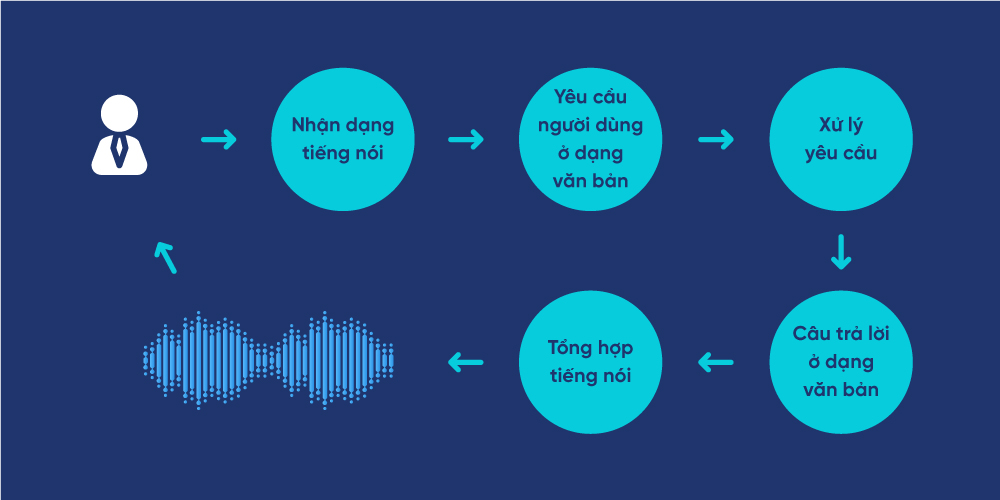
\includegraphics[width=1\textwidth]{
		nlp.jpg
	}
	\caption[Kiến trúc của một chương trình máy tính giao tiếp với con người thông qua tiếng nói ]{
		Kiến trúc của một chương trình máy tính giao tiếp với con người thông qua tiếng nói \label{pic1.1}
	}
\end{figure}


\begin{itemize}
	\item  Nhận dạng tiếng nói: ở bước này, máy tính sẽ nhận dạng yêu cầu của người dùng ở dạng tiếng nói và chuyển yêu cầu này về dạng văn bản.
	\item Xử lý yêu cầu: máy tính sẽ phân tích yêu cầu ở dạng văn bản, xử lý, đưa ra câu trả lời sử dụng các kỹ thuật trong xử lý văn bản.
	\item Tổng hợp tiếng nói: ở bước này, câu trả lời sẽ được chuyển từ dạng văn bản sang tiếng nói và gửi tới người dùng.
\end{itemize}


\section{Các bài toán cơ bản trong NLP } 
---------------------------------
\subsection{Mô hình hóa ngôn ngữ (Language modelling)}
Mô hình hóa ngôn ngữ (LM) gán một xác suất cho bất kỳ chuỗi từ nào. Về cơ bản, trongbài toán này, ta cần dự đoán từ tiếp theo xuất hiện theo trình tự, dựa trên lịch sử của các từ đã xuất hiện trước đó. LM rất quan trọng trong các ứng dụng khác nhau của NLP, và là lý do tại sao máy móc có thể hiểu được thông tin định tính. Một số ứng dụng của Mô hình hóa ngôn ngữ bao gồm: nhận dạng giọng nói, nhận dạng ký tự quang học, nhận dạng chữ viết tay, dịch máy và sửa lỗi chính tả.\cite{WEBSITE:3}

\subsection{Phân loại văn bản (Text classification)}
Phân loại văn bản gán các danh mục được xác định trước cho văn bản dựa trên nội dung của nó. Cho đến nay, phân loại văn bản là ứng dụng phổ biến nhất của NLP, được sử dụng để xây dựng các công cụ khác nhau như trình phát hiện thư rác và chương trình phân tích cảm xúc.\cite{WEBSITE:3}

\subsection{Trích xuất thông tin (Information extraction)}
Trích xuất thông tin (IE) tự động trích xuất thông tin có liên quan từ các tài liệu văn bản không có cấu trúc và / hoặc bán cấu trúc. Ví dụ về các loại tài liệu này bao gồm lịch sự kiện từ email hoặc tên của những người được đề cập trong một bài đăng trên mạng xã hội.\cite{WEBSITE:3}

\subsection{Truy xuất thông tin (Information retrieval)}
Google là một loại hệ thống Truy xuất Thông tin (IR) phổ biến nhất mà chúng ta thường sử dụng. IR làm nhiệm vụ tìm kiếm các tài liệu có liên quan từ một bộ dữ liệu lớn các tài liệu liên quan đến truy vấn do người dùng thực hiện.\cite{WEBSITE:3}

\subsection{Tác tử phần mềm hội thoại (Conversational agent)}
Tác tử phần mềm hội thoại thuộc AI hội thoại, liên quan đến việc xây dựng các hệ thống đối thoại mô phỏng các tương tác của con người. Các ví dụ phổ biến về AI hội thoại bao gồm Alexa, Siri, Google Home, Cortana, hay trợ lý ảo ViVi. Các công nghệ như chatbot cũng được hỗ trợ bởi  tác tử phần mềm hội thoại và ngày càng phổ biến trong các doanh nghiệp.\cite{WEBSITE:3}

\subsection{Tóm tắt văn bản (Text summarization)}
Tự động tóm tắt là quá trình rút ngắn một tập hợp dữ liệu để tạo một tập hợp con đại diện cho thông tin quan trọng nhất hoặc có liên quan trong nội dung gốc.\cite{WEBSITE:3}

\subsection{Hỏi đáp (Question answering)}
Hỏi đáp là bài toán xây dựng các hệ thống có thể tự động trả lời cho các câu hỏi do con người đặt ra bằng ngôn ngữ tự nhiên.\cite{WEBSITE:3}

\subsection{Dịch máy (Machine translation)}
Dịch máy (MT) là một nhánh con của ngôn ngữ học tính toán liên quan đến việc chuyển đổi một đoạn văn bản từ ngôn ngữ này sang ngôn ngữ khác. Một ứng dụng phổ biến của loại này là Google Dịch.\cite{WEBSITE:3}

\subsection{Mô hình hóa chủ đề (Topic modelling)}
Mô hình hóa chủ đề là một kỹ thuật Học máy không giám sát giúp khám phá cấu trúc chủ đề của một bộ tài liệu lớn. Ứng dụng NLP này là một công cụ khá phổ biến, được sử dụng trên nhiều lĩnh vực khác nhau – như Văn học, và Tin sinh học.\cite{WEBSITE:3}


%----------------------------------------------------------------------------------------

\section{Các công cụ giải quyết các bài toán NLP} 
\subsection{NLTK}
Natural Language ToolKit (NLTK) là một trong những nền tảng hàng đầu để xây dựng các chương trình Python xử lý và phân tích dữ liệu ngôn ngữ của con người. 

NLTK cung cấp giao diện dễ sử dụng cho hơn 50 tài nguyên ngữ liệu và từ vựng như mạng từ, cùng với một bộ thư viện xử lý văn bản để phân loại, mã hóa, tạo gốc, gắn thẻ, phân tích cú pháp và lập luận ngữ nghĩa.\cite{WEBSITE:3}

Ví dụ về sử dụng NLTK để xử lí dữ liệu

\lstinputlisting[style=codePython]{"Code/nltk.py"}

Kết quả:

\lstinputlisting[style=plaintext]{"Code/nltk_result.txt"}

\subsection{Spacy}
Bản phát hành đầu tiên của SpaCy là vào tháng 2 năm 2015, khiến nó trở thành một trong những framework nguồn mở gần đây dành cho các ứng dụng Xử lý ngôn ngữ tự nhiên Python. So với NLTK được tạo ra vào năm 2001, những người sáng tạo SpaCy có đủ thời gian để tìm hiểu NLTK và xem nó còn thiếu ở đâu. Một trong những cải tiến dễ nhận biết nhất so với NTLK bao gồm các cải tiến về hiệu suất, vì SpaCy sử dụng một số thuật toán mới nhất và tốt nhất.

Ngoài ra, SpaCy được ghi chép rất đầy đủ và được thiết kế để hỗ trợ khối lượng lớn dữ liệu. Nó cũng bao gồm một loạt các mô hình Xử lý ngôn ngữ tự nhiên được đào tạo trước, giúp việc học, giảng dạy và thực hành Xử lý ngôn ngữ tự nhiên với SpaCy trở nên dễ tiếp cận hơn \cite{WEBSITE:3}. 

Ví dụ tách chuỗi bằng spacy:

\lstinputlisting[style=codePython]{"Code/spacy.py"}

Ví dụ đọc dữ liệu từ file sau đó xử lí:

\lstinputlisting[style=codePython]{"Code/spacy1.py"}

Kết quả: 

\lstinputlisting[style=plaintext]{"Code/spacy_result.txt"}

\subsection{Stanford CoreNLP}
CoreNLP là một thư viện cực kỳ phổ biến cho các tác vụ Xử lý Ngôn ngữ tự nhiên, được xây dựng bởi cộng đồng NLP Stanford. Ngược lại với NLTK và SpaCy, được viết bằng Python hoặc Cython tương ứng, CoreNLP bằng Java – có nghĩa là máy tính của bạn sẽ cần phải có JDK (nhưng nó có API cho hầu hết các ngôn ngữ lập trình).

Trên trang chủ CoreNLP, các nhà phát triển mô tả CoreNLP là “nơi duy nhất để xử lý ngôn ngữ tự nhiên trong Java! CoreNLP cho phép người dùng lấy các chú thích ngôn ngữ cho văn bản, bao gồm mã thông báo và ranh giới câu, các phần của giọng nói, các thực thể được đặt tên, giá trị số và thời gian, trình phân tích cú pháp phụ thuộc và ý kiến chính, tình cảm, phân bổ trích dẫn và quan hệ. CoreNLP hiện hỗ trợ 6 ngôn ngữ: Ả Rập, Trung Quốc, Anh, Pháp, Đức và Tây Ban Nha.

Một trong những ưu điểm chính của CoreNLP là nó có khả năng mở rộng rất cao, trở thành lựa chọn phù hợp cho các tác vụ phức tạp. Một yếu tố khác là CoreNLP được xây dựng chú trọng đến tốc độ – nó được tối ưu hóa để vận hành cực kỳ nhanh. \cite{WEBSITE:3}

Ví dụ sử dụng Standford CoreNlp:

\lstinputlisting[style=codePython]{"Code/StandfordNLP.py"}

Kết quả:

\lstinputlisting[style=plaintext]{"Code/coreNLP-result.txt"}

\subsection{Gensim}
Gensim là một framework Python mã nguồn mở chuyên dụng, được sử dụng để biểu diễn tài liệu dưới dạng vectơ ngữ nghĩa theo những cách hiệu quả nhất và dễ dàng nhất có thể. Các tác giả đã thiết kế Gensim để xử lý văn bản thô, không có cấu trúc bằng cách sử dụng nhiều thuật toán học máy – vì vậy sử dụng Gensim để tiếp cận các tác vụ như Lập mô hình chủ đề là một ý tưởng tốt. Thêm vào đó, Gensim làm rất tốt việc xác định các điểm tương đồng trong văn bản, lập chỉ mục văn bản và điều hướng các tài liệu khác nhau.\cite{WEBSITE:3}

Gensim được xây dựng vì 3 lý do:

\begin{itemize}
	\item Tính thực tiễn – tập trung vào các thuật toán đã được chứng minh, đã được kiểm chứng để giải quyết các vấn đề thực tế của ngành. Gensim tập trung nhiều hơn vào kỹ thuật, ít hơn về học thuật.
	\item Độc lập đối với bộ nhớ – không cần toàn bộ kho dữ liệu đào tạo phải nằm hoàn toàn trong RAM cùng một lúc. Nó có thể xử lý kho dữ liệu lớn, quy mô web bằng cách sử dụng luồng dữ liệu.
	\item Hiệu suất – triển khai tối ưu hóa cao các thuật toán không gian vectơ phổ biến sử dụng C, BLAS và ánh xạ bộ nhớ
\end{itemize}

Ví dụ sử dụng Gensim:

\lstinputlisting[style=codePython]{"Code/gensim.py"}

Kết quả:

\lstinputlisting[style=plaintext]{"Code/gensim-result.txt"}
%----------------------------------------------------------------------------------------



			
			
			
 
%\chapter{Feature Engineering và các model xử lý dữ liệu dạng văn bản}
 % Tên của chương
 \label{Chapter2}

\section{Các bước xử lý một bài toán học máy (MLP)}
Bất kỳ hệ thống thông minh nào về cơ bản đều bao gồm các bước bắt đầu từ việc nhập dữ liệu thô, sử dụng các kỹ thuật để sắp xếp, xử lý, thiết kế các đặc trưng (feature) và thuộc tính có ý nghĩa từ dữ liệu này. Sau đó, chúng ta thường sử dụng các kỹ thuật như mô hình thống kê hoặc các mô hình học máy để xây dựng các mô hình với mục đích giải quyết yêu cầu đặt ra. Một quy trình tiêu chuẩn điển hình dựa trên mô hình tiêu chuẩn công nghiệp CRISP-DM được mô tả như hình \ref{pic2.1}

\begin{figure}[h!]
	\centering
	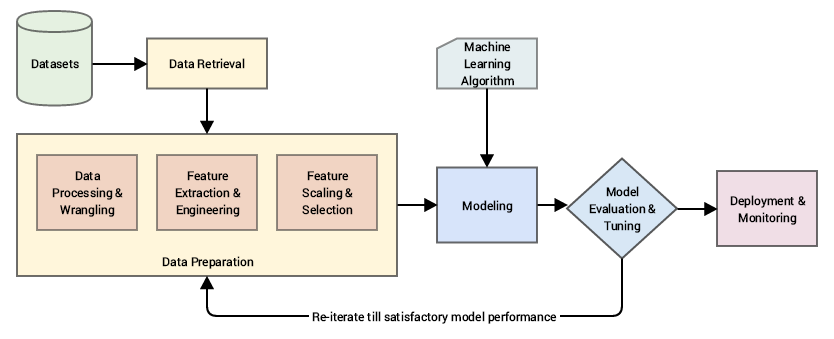
\includegraphics[width=1\textwidth]{
		mlp.png
	}
	\caption[Mô hình tiêu chuẩn công nghiệp CRISP-DM]{
		Mô hình tiêu chuẩn công nghiệp CRISP-DM \label{pic2.1}
	}
\end{figure}

\section{Giới thiệu về Feature Engineering}
Feature Engineerning là một giai đoạn không thể thiếu trong quá trình phát triển bất kỳ một hệ thống thông minh nào. Mặc dù hiện nay chúng ta có rất nhiều các phương pháp mới như học sâu, siêu mô hình hỗ trợ học máy tự động (automated machine learning), tuy nhiên với mỗi vấn đề cụ thể cần giải quyết luôn có những đặc trưng quan trọng hơn, có giá trị hơn để quyết định hiệu suất hệ thống của bạn.


\section{Cơ bản về đặc trưng của dữ liệu}

Một đặc trưng (feature) thường là một đại diện cụ thể trên dòng đầu tiên của dữ liệu thô, là một thuộc tính riêng lẻ, có thể đo lường và mô tả bởi một cột trong tập dữ liệu. Lấy ví dụ với một tập dữ liệu hai chiều, mỗi observation (quan sát) được mô tả bởi một hàng và mỗi đặc trưng được mô tả bởi một cột, sẽ có giá trị cụ thể cho mỗi đặc trưng của từng quan sát như hình \ref{pic2.2}

\begin{figure}[h!]
	\centering
	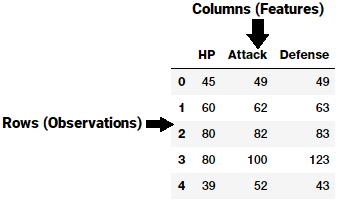
\includegraphics[width=0.5\textwidth]{
		featuresData.png
	}
	\caption[Đặc trưng của dữ liệu]{
		Đặc trưng của dữ liệu \label{pic2.2}
	}
\end{figure}

Như ví dụ ở hình trên, mỗi hàng thường biểu thị một vectơ đặc trưng và tập hợp tất cả các đặc trưng trên tất cả các quan sát tạo thành một ma trận hai chiều còn được gọi là feature-set. Thông thường, các thuật toán học máy hoạt động với các ma trận số hóa hoặc tenxo bởi vậy hầu hết các kỹ thuật feature engineering sẽ xử lý việc chuyển đổi dữ liệu thô thành các dạng biểu diễn số học giúp các thuật toán có thể dễ dàng hiểu được.

Các đặc trưng có thể chia thành hai loại chính:

\begin{itemize}
	\item \textbf{Đặc trưng thô (Raw features)}: là các đặc trưng vốn có được lấy trực tiếp từ tập dữ liệu mà không cần sử dụng thêm thao tác kỹ thuật nào
	\item \textbf{Đặc trưng phát sinh (Derived features)}: là các đặc trưng được thu được sau quá trình feature engineering, là kết quả của quá trình trích xuất và xử lý các đặc trưng có sẵn. 
\end{itemize}

\section{Kĩ thuật tạo đặc trưng dữ liệu}

Về kĩ thuật tạo đặc trưng cho dữ liệu có 3 phương pháp chính:
\begin{itemize}
	\item \textbf{Trích lọc feature}: Không phải toàn bộ thông tin được cung cấp từ một biến dự báo hoàn toàn mang lại giá trị trong việc phân loại. Do đó chúng ta cần phải trích lọc những thông tin chính từ biến đó. Chẳng hạn như trong các mô hình chuỗi thời gian chúng ta thường sử dụng kĩ thuật phân rã thời gian để trích lọc ra các đặc trưng như Ngày thành Năm, Tháng, Quí,…. Các đặc trưng mới sẽ giúp phát hiện các đặc tính chu kì và mùa vụ, những đặc tính mà thường xuất hiện trong các chuỗi thời gian
	\item \textbf{Biến đổi feature}:  Biến đổi dữ liệu gốc thành những dữ liệu phù hợp với mô hình nghiên cứu. Những biến này thường có tương quan cao hơn đối với biến mục tiêu và do đó giúp cải thiện độ chính xác của mô hình
	\item \textbf{Lựa chọn feature} : Phương pháp này được áp dụng trong những trường hợp có rất nhiều dữ liệu mà chúng ta cần lựa chọn ra dữ liệu có ảnh hưởng lớn nhất đến sức mạnh phân loại của mô hình. Các phương pháp có thể áp dụng đó là ranking các biến theo mức độ quan trọng bằng các mô hình như Random Forest, Linear Regression, Neural Network,…; Sử dụng chỉ số IV trong scorecard; Sử dụng các chỉ số khác như AIC hoặc Pearson Correlation, phương sai.
\end{itemize}

\section{Xử lý dữ liệu dạng văn bản}

\begin{enumerate}
	\item Import các thư viện cần thiết và khởi tạo một đoạn văn bản mẫu cần xử lý \lstinputlisting[style=codePython]{"Code/dependencies.py"}
	Kết quả: 
	\lstinputlisting[style=plaintext]{"Code/dependencies.txt"}
	\item
	\item Tiền xử lý văn bản \cite{WEBSITE:10}
	\begin{itemize}
		\item \textbf{Xóa thẻ tags}: Văn bản chúng ta gặp thường chứa nội dung không cần thiết như các thẻ \textbf{HTML}, không có giá trị khi phân tích. Thư viện \textbf{BeautifulSoup} là một công cụ tuyệt vời và cần thiết để xử lý trong trường hợp này.
		\item \textbf{Xóa các ký tự có dấu}:Trong bất kỳ văn bản nào, đặc biệt nếu bạn đang xử lý ngôn ngữ tiếng Anh, thường các bạn cần phải xử lý các ký tự có dấu. Do đó, chúng ta vần đảm bảo rằng các ký tự này cần được chuyển đổi và chuẩn hóa thành các ký tự ASCII
		\item \textbf{Biến đổi các từ viết tắt}: Trong tiếng Anh, các từ viết tắt về cơ bản là phiên bản rút gọn của các từ hoặc âm tiết. Những từ viết tắt của các từ hoặc cụm từ thường được tạo ra bằng cách loại bỏ các chữ cái và âm tiết. Ví dụ như: \textbf{do not -> don't, I would -> I'd}. Chuyển đổi từ dạng viết tắt thành dạng đầy đủ cũng là một bước cần thiết để chuẩn hóa văn bản.
		\item \textbf{Xóa các ký tự đặc biệt}: Các ký tự đặc biệt thường là các ký tự không phải là chữ và số, thường gây "nhiễu" cho dữ liệu của chúng ta. Thông thường, regular expressions \textbf{(regexes)} có thể được sử dụng để xử lý vấn đề này.
		\item \textbf{Từ gốc và ngữ pháp}:  Trong các ngữ cảnh khác nhau, các từ gốc thường được gắn thêm các tiền tố và hậu tố vào để đúng với ngữ pháp. Ví dụ các từ: \textbf{WATCHES, WATCHING}, and \textbf{WATCHED}. Chúng ta có thể thấy rằng chúng đều có chung từ gốc là \textbf{WATCH}.
		\item \textbf{Xóa các stopwords}: stopwords là các từ có ít hoặc không có ý nghĩa gì đặc biệt khi xây dựng các đặc trưng
	\end{itemize}
	\lstinputlisting[style=codePython]{"Code/simpleDataProcessing.py"}
	
	Kết quả:
	
	\lstinputlisting[style=plaintext]{"Code/simpleDataProcessing.txt"}

\end{enumerate}

\section{Các model phổ biến trong việc xử lý dữ liệu dạng văn bản}

\subsection{Bag of Words Model - Túi từ}
Mô hình Bag of words biểu diễn cho mỗi mẫu dữ liệu văn bản dưới dạng một vecto số trong đó mỗi chiều là một từ cụ thể trong kho dữ liệu và giá trị có thể là tần số của nó xuất hiện trong đoạn văn bản (giá trị có thể là 0 hoặc 1) hoặc thậm chí là các giá trị có trọng số. \cite{WEBSITE:10}

Tên mô hình này là Bag of words thể hiện theo đúng nghĩa đen của nó nghĩa là một túi các từ, không quan tâm đến trật tự, trình tự, ngữ pháp. \cite{WEBSITE:10}

Ví dụ về model \textbf{Bag of Words}

\lstinputlisting[style=codePython]{"Code/bagOfWords.py"}

Kết quả
\lstinputlisting[style=plaintext]{"Code/bagOfWords.txt"}

\subsection{Bag of N-Grams}
Là phân bố xác suất trên các tập văn bản\\

Cho biết xác suất của 1 câu (hoặc 1 cụm từ) thuộc 1 ngôn ngữ là bao nhiêu
Mô hình ngôn ngữ tốt sẽ đánh giá đúng các câu đúng ngữ pháp, trôi chảy hơn các cụm từ có thứ tự ngẫu nhiên \cite{NGRAM1}

Các mô hình N-grams phổ biến \cite{NGRAM}:
\begin{itemize}
	\item \textbf{Unigram}: mô hình với n=1, tức là ta sẽ tính tần suất xuất hiện của một kí tự (từ), như: “k”, “a”,…
	\item \textbf{Bigrams}: với n=2 , là mô hình được sử dụng nhiều trong việc phân tích các hình thái cho ngôn ngữ
	\item \textbf{Trigrams}:với n-3, với n càng lớn thì độ chính xác càng cao tuy nhiên đi kèm với đó thì độ phức tạp cũng lớn hơn
\end{itemize}

Mô hình N-gram \cite{NGRAM}:
Mục tiêu: Tính xác suất của 1 câu hoặc 1 cụm từ:
\begin{itemize}
	\item Để tính xác suất của một câu: W1W2...Wk...Wn, Theo công thứ Bayes \cite{NGRAM} \ref{2.1}:
	\begin{equation}
		p(w_1...w_n) = \frac{count(w_1...w_n)}{N} \label{2.1} 
	\end{equation}
	
	\item Tuy nhiên, công thức trên có độ phức tạp lớn, vì vậy người ta thường sử dụng công thức Markov \cite{NGRAM} \ref{2.2}:
	\begin{equation}
		p(w_1...w_n) = p(w_1) * p(w_2|w_1) * p(w_3|w_1w_2)  *...*p(w_n|w_1...w_(n-1)) \label{2.2} 
	\end{equation}
\end{itemize}

Ví dụ về model \textbf{Bag of N-grams}:

\lstinputlisting[style=codePython]{"Code/nGram.py"}

Kết quả \ref{pic2.3}: 
\begin{figure}[h!]
	\centering
	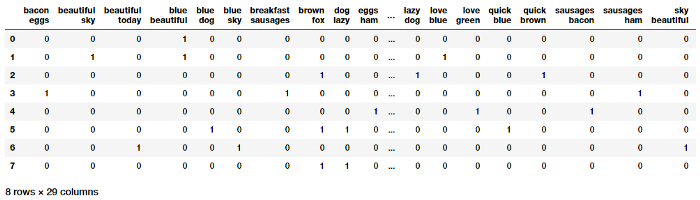
\includegraphics[width=1\textwidth]{
			ngramFigures.png
		}
	\caption[Kết quả của model Bag of N-grams]{
			Kết quả của model Bag of N-grams  \cite{WEBSITE:11} \label{pic2.3}
		}
\end{figure}

\subsection{TF-IDF - Term Frequency-Inverse Document Frequency}
TF-IDF là viết tắt của Term Frequency-Inverse Document Frequency.\\
Hiểu một cách đơn giản nó là sự kết hợp của tần số xuất hiện của một từ trong một mẫu và nghịch đảo của tần số của từ đó trong toàn bộ tập dữ liệu\\
Kỹ thuật này được phát triển để đánh giá kết quả cho các truy vấn trong công cụ tìm kiếm và hiện tại nó là một phần không thể thiếu trong xử lý ngôn ngữ tự nhiên \cite{WEBSITE:11}\\
Về mặt toán học có thể định nghĩa như sau \cite{WEBSITE:10} \ref{2.3}:

\begin{equation}
	tfidf(w,D) = tf(w,D)*idf(w,D)=tf(w,D)*log(\frac{C}{df(w)}) \label{2.3}
\end{equation}

Theo công thức trên, \textbf{tfidf(w,D)} là một 'score'. TF-IDF cho từ \textbf{w} trong mẫu \textbf{D}. Thuật ngữ \textbf{tf(w,D)} đại diện cho tần số của từ \textbf{w} xuất hiện trong mẫu \textbf{D} có thể lấy được từ mô hình \textbf{Bag of words}. Thuật ngữ \textbf{idf(w,D)} là tần số nghịch đảo của \textbf{w} có thể tính là \textbf{log} của tổng số mẫu dữ liệu xuất hiện từ \textbf{w}. \\
Mô hình này có thể có rất nhiều biến thể khác nhau, tuy nhiên chúng đều cho kết quả khá giống nhau. 

Ví dụ về model \textbf{TF-IDF}: 

\lstinputlisting[style=codePython]{"Code/tfidf.py"}

Kết quả \ref{pic2.4}:

\begin{figure}[h!]
	\centering
	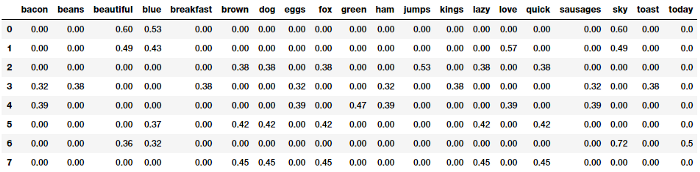
\includegraphics[width=1\textwidth]{
		tfidfFigures.png
	}
	\caption[Kết quả của model TF-IDF]{
		Kết quả của model TF-IDF   \cite{WEBSITE:11} \label{pic2.4}
	}
\end{figure}

\subsection{Document Similarity}
Document Similarity (hay độ tương tự của văn bản) là quá trình sử dụng số liệu dựa trên khoảng cách hoặc độ tương tự có thể sử dụng để xác định mức độ tương đương của một văn bản với bất kỳ văn bản nào khác dựa trên các đặc trưng được trích xuất ra từ \textbf{bag of words} hoặc \textbf{tf-idf}.\\
Sự tương tự giữa các mẫu dữ liệu trong một kho văn bản cũng được hiểu là sự tương tự giữa từng cặp mẫu trong toàn bộ kho văn bản đó

Có rất nhiều công thức có thể sử dụng để tính toán độ tương tự này như khoảng cách cosin, khoảng cách euclide, khoảng cách manhattan...  \cite{WEBSITE:11}

Ví dụ sử dụng \textbf{cosine} để tính toán độ tương tự 
\lstinputlisting[style=codePython]{"Code/cosine.py"}

Kết quả \ref{pic2.5}:
\begin{figure}[h!]
	\centering
	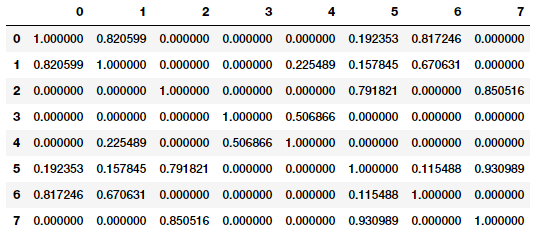
\includegraphics[width=1\textwidth]{
		cosine.png
	}
	\caption[Kết quả của model  Document Similarity.]{
		Kết quả của model  Document Similarity.   \cite{WEBSITE:11} \label{pic2.5}
	}
\end{figure}

Về cơ bản, khoảng cách cosin cung cấp cho chúng ta một số liệu biểu thị góc giữa 2 vecto đặc trưng tương ứng của từng mẫu. Góc giữa hai mẫu càng gần nhau thì độ tương tự của hai mẫu đó càng lớn như được mô tả trong hình dưới đây\\

\begin{figure}[h!]
	\centering
	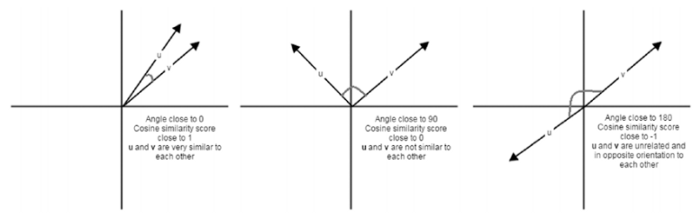
\includegraphics[width=1\textwidth]{
		cosin1.png
	}
	\caption[Độ tương tự của hai mẫu theo khoảng cách cosine]{
		Độ tương tự của hai mẫu theo khoảng cách cosine.   \cite{WEBSITE:11} \label{pic2.5}
	}
\end{figure}
%
%\section{Trích lọc đặc trưng cho dữ liệu dạng văn bản}
%
%Dữ liệu văn bản có thể đến từ nhiều nguồn và nhiều định dạng khác nhau (kí tự thường, kí tự hoa, kí tự đặc biệt,…). Có nhiều phương pháp xử lý dữ liệu phù hợp với từng đề tài cụ thể. Ở đây chúng tôi sẽ sử dụng kĩ thuật mã hóa (tokenization)\cite{WEBSITE:3}
%
%Mã hóa đơn giản là việc chúng ta chia đoạn văn thành các câu văn, các câu văn thành các từ. 
%
%Trong mã hóa thì từ là đơn vị cơ sở. Chúng ta cần một bộ tokenizer có kích thước bằng toàn bộ các từ xuất hiện trong văn bản hoặc bằng toàn bộ các từ có trong từ điển. 
%
%Một câu văn sẽ được biểu diễn bằng một sparse vector mà mỗi một phần tử đại diện cho một từ, giá trị của nó bằng 0 hoặc 1 tương ứng với từ không xuất hiện hoặc có xuất hiện.
%
%Chúng ta sử dụng các túi từ (bags of words) để tạo ra một vector có độ dài bằng độ dài của tokenizer và mỗi phần tử của túi từ sẽ đếm số lần xuất hiện của một từ trong câu và sắp xếp chúng theo một vị trí phù hợp trong vector. Bên dưới là code minh họa cho quá trình này.
%
%\lstinputlisting[style=codePython]{"Code/tokenization.py"}
%
%Quá trình này có thể được mô tả như hình \ref{pic2.3}:
%\begin{figure}[h!]
%	\centering
%	\includegraphics[width=1\textwidth]{
%		tokenization.png
%	}
%	\caption[Biểu diễn kĩ thuật mã hóa]{
%		Biểu diễn kĩ thuật mã  \label{pic2.3}
%	}
%\end{figure}
%
%Cách biểu diễn theo túi từ có hạn chế đó là chúng ta không phân biệt được 2 câu văn có cùng các từ bởi túi từ không phân biệt thứ tự trước sau của các từ trong một câu. Chặng như ‘you have no dog’ và ‘no, you have dog’ là 2 câu văn có biểu diễn giống nhau mặc dù có ý nghĩa trái ngược nhau. Chính vì thế phương pháp N-gram sẽ được sử dụng thay thế.
%
%\lstinputlisting[style=codePython]{"Code/nGram.py"}
%
%
%Những từ hiếm khi được tìm thấy trong tập văn bản (corpus) nhưng có mặt trong một văn bản cụ thể có thể quan trọng hơn. Do đó cần tăng trọng số của các nhóm từ ngữ để tách chúng ra khỏi các từ phổ biến. Cách tiếp cận này được gọi là TF-IDF (Term Frequency - Inverse Document Frequency)
%
%Các chỉ số chính đánh giá tần xuất xuất hiện của một từ trong toàn bộ tập văn bản là idf và tfidf được tính theo công thức \ref{tdf} \ref{tfidf}:
%
%\begin{equation}
%	idf(t,D) = log(\frac{|D|}{df(d,t) + 1})\\ \label{tdf}
%\end{equation}
%
%\begin{equation}
%	tfidf(t,d,D) = tf(d,d) x idf(i, D) \label{tfidf}
%\end{equation}
%
%Ở đây:
%\begin{itemize}
%	\item \textbf{|D|}: là số lượng các văn bản trong tập văn bản
%	\item \textbf{df(d,t)}: là số lượng các văn bản là từ t xuất hiện
%	\item \textbf{tf(dt)}: là tần suất các từ xuất hiện trong một văn bản
%\end{itemize}
%Như vậy một từ càng phổ biến khi idf càng nhỏ và tfidf càng lớn.
%Do đó để tính \textbf{tfidf} cho các từ trong văn bản, ta có thể làm như sau:
%
%\lstinputlisting[style=codePython]{"Code/tfidf.py"}
%
%Kết quả:
%
%\lstinputlisting[style=plaintext]{"Code/tfidf.txt"}
%
%Ta có thể thấy từ "I" xuất hiện ở toàn bộ các câu và không mang nhiều ý nghĩa của chủ đề của câu nên có thể coi là một stopword. Bằng phương pháp lọc cận trên của tần suất xuất hiện từ trong văn bản là 90\% ta đã loại bỏ được từ này khỏi dictionary.
%\chapter{Topic Modeling}
\label{Chapter3}
\section{Topic Modeling là gì ?}
\begin{figure}[h!]
	\centering
	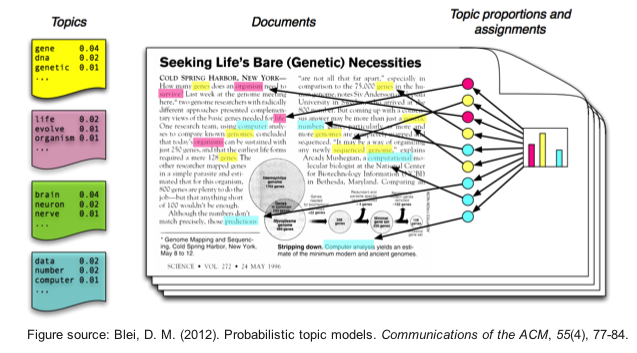
\includegraphics[width=1\textwidth]{
		topicModeling.png
	}
	\caption[Topic Modeling]{
		Topic Modeling   \cite{WEBSITE:11}
	}
\end{figure}
Topic modeling hay Mô hình hóa chủ đề là một kĩ thuật học máy tự động phân tích dữ liệu văn bản để xác định các từ cụm cho một tập hợp các tài liệu. Điều này được gọi là học máy 'không giám sát' vì nó không yêu cầu dữ liệu  được con người phân loại trước đây.

Ý tưởng về các topic models xoay quanh quá trình sắp xếp các văn bản vào những dạng chủ đề, khái niệm. 

Mỗi chủ để được biểu diễn dưới dạng là tập hợp của các từ/thuật ngữ có trong kho văn bản.

Nếu chúng xuất hiện cùng với nhau các từ/thuật ngữ này sẽ biểu thị, tượng trưng cho một chủ đề hoặc khái niệm cụ thể. Chúng ta có thể dễ dạng phân biệt các chủ đề với nhau nhờ ngữ nghĩa của các thuật ngữ đó

Tuy nhiên, các chủ đề thường có sự chồng chéo nhất định trên dữ liệu. Các topic models sẽ cực kỳ hữu ích trong việc tóm tắt, rút gọn khối lượng lớn tài liệu, văn bản để trích xuất, mô tả các khái niệm chính nhất. Chúng cũng hữu ích trong việc trích xuất các đặc trưng từ dữ liệu văn bản để nắm bắt các pattern tiềm ẩn trong dữ liệu đó. \cite{WEBSITE:12}



\section{Các kỹ thuật sửu dụng trong Topic Modeling}

Có nhiều kỹ thuật khác nhau để mô hình hóa chủ đề văn bản và hầu hết chúng liên quan đến một số dạng phân tách ma trận

Một số kỹ thuật như \cite{WEBSITE:11}:

\begin{enumerate}
	\item \textbf{Latent Semantic Analysis  (LSA) - Phân tích ngữ nghĩa tiềm ẩn} :sử dụng các phương pháp phân tách ma trận, cụ thể hơn là phân tách các giá trị đơn lẻ.
	\item \textbf{Latent Dirichlet Allocation (LDA) - Phân bố Dirichlet tiền ẩn}: một kỹ thuật sử dụng mô hình xác suất tổng quát trong đó mỗi mẫu tài liệu bao gồm một sự kết hợp của một số chủ đề và mỗi thuật ngữ hoặc từ có thể được gán cho một chủ đề cụ thể.
\end{enumerate}

\subsection{Latent Semantic Analysis (LSA)}

LSA (Phân tích ngữ nghĩa tiềm ẩn) còn được gọi là LSI (Chỉ số ngữ nghĩa tiềm ẩn) LSA sử dụng mô hình túi từ (BoW). 
Hàng và cột đại diện cho tài liệu. \\
LSA học các chủ đề tiềm ẩn bằng cáchsử dụng các phương pháp phân tách ma trận, cụ thể hơn là phân tách các giá trị đơn lẻ.

\textbf{Singular Value Decomposition(SVD)}
SVD là một phương pháp phân tích ma trận thành nhân tử đại diện cho một ma trận trong tích của hai ma trận \ref{equa1} \cite{WEBSITE:13}

\begin{equation}
	M=U \sum V^* \label{equa1}
\end{equation}
Trong đó:
\begin{itemize}
	\item M: là ma trận cỡ mxm\\
	\item U: là ma trận cỡ mxn phía bên trái\\
	\item V: là ma trận cỡ mxn phía bên phải\\
	\item V*: là ma trận chuyển vị của ma trận V\\
\end{itemize}

\textbf{Thực nghiệm thuật LSA sử dụng Gensim} \cite{WEBSITE:13}
\begin{enumerate}
	\item \textbf{Import các thư viện cần thiết}
		\lstinputlisting[style=codePython]{"Code/dependencies1.py"}
	\item \textbf{Load dữ liệu mẫu}:
		\lstinputlisting[style=codePython]{"Code/loadData.py"}
	
	\item \textbf{Tiền xử lý dữ liệu}:
		\lstinputlisting[style=codePython]{"Code/preprocessing.py"}
		
	\item \textbf{Chuẩn bị các dữ liệu dạng văn bản}:
		\lstinputlisting[style=codePython]{"Code/prepareCorpus.py"}
		
	\item \textbf{Khởi tạo model LSA sử dụng Gensim}:
		\lstinputlisting[style=codePython]{"Code/lsaGensim.py"}
		
	\item \textbf{Xác định số lượng topics}: 
		\lstinputlisting[style=codePython]{"Code/determineTopics.py"}
	\item \textbf{Kết quả thực nghiệm} :
		\lstinputlisting[style=plaintext]{"Code/resultLSA.txt"}
		\begin{figure}[h!]
			\centering
			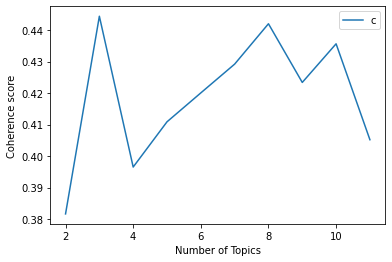
\includegraphics[width=1\textwidth]{
				resultLSA.png
			}
			\caption[Kết quả thuật toán LSA trong Topic Modeling]{
				Kết quả thuật toán LSA trong Topic Modeling 
			}
		\end{figure}
\end{enumerate}

\subsection{Latent Dirichlet Allocation (LDA)}
Model LDA là lớp mô hình sinh (generative model) cho phép xác định một tợp hợp các chủ đề tưởng tượng (imaginary topics) mà mỗi topic sẽ được biểu diễn bởi tập hợp các từ. Mục tiêu của LDA là mapping toàn bộ các văn bản sang các topics tương ứng sao cho các từ trong mỗi một văn bản sẽ thể hiện những topic tưởng tượng ấy.

\textbf{Ứng dụng của gensim trong bài toán LDA} \cite{WEBSITE:14}

Dữ liệu được sử dụng là 20-newgroups dataset

Dữ liệu bao gồm 11k các posts liên quan đến 20 chủ đề khác nhau đã được gán nhãn.

\begin{enumerate}
	\item \textbf{Import các thư viện cần thiết}
	\lstinputlisting[style=codePython]{"Code/importData.py"}
	
	\item \textbf{Dữ liệu mẫu} %\ref{tab:data}:
	\lstinputlisting[style=plaintext]{"Code/loadDataRes.txt"}
	
%	\begin{table}[h!]
%		\caption{Dữ liệu mẫu: }
%		\label{tab:data}
%		\centering
%		\begin{tabular}{l l l 1}
%			\toprule
%			\tabhead{No}&\tabhead{content}&\tabhead{target}&\tabhead{target_names}\\
%			\midrule
%			0 & From: lerxst@wam.umd.edu (where's my thing)... & 7 & rec.autos\\
%			1 & From: guykuo@carson.u.washington.edu (Guy Kuo)... & 4 & comp.sys.mac.hardware\\
%			10 & From: guykuo@carson.u.washington.edu (Guy Kuo)... & 8 & rec.motorcycles\\
%			100 & From: guykuo@carson.u.washington.edu (Guy Kuo)... & 6 & misc.forsale\\
%			1000 & 	From: dabl2@nlm.nih.gov (Don A.B. Lindbergh)... & 2 & comp.os.ms-windows.misc\\
%			\bottomrule \\
%		\end{tabular}
%	\end{table}
	
	\item \textbf{Visualization số lượng các topics}:
		\begin{figure}[h!]
			\centering
			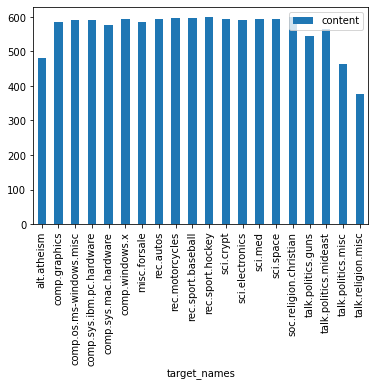
\includegraphics[width=1\textwidth]{
				output.png
			}
			\caption[Visualization số lượng các topics]{
				Visualization số lượng các topics
			}
		\end{figure}
		Như vậy có 20 nhóm, mỗi nhóm có số lượng các posts trong khoảng từ 400-600. phân về các chủ đề như: auto, mobile, medicine,….
	\newpage
	\item \textbf{Tiền xử lý dữ liệu}:
	\lstinputlisting[style=codePython]{"Code/preprocessing1.py"}
	\textbf{Kết quả}:
	\lstinputlisting[style=plaintext]{"Code/preprocessing1Res.txt"}
	
	\item \textbf{Tạo ra các bigram và trigram}:
	Hiện tại các từ vựng đang gồm toàn bộ là những từ đơn. Để tăng độ chính xác cho mô hình ta sẽ cần gom cụm các từ đơn có tần xuất xuất hiện cùng nhau chung thành những collocations có độ dài gồm 2 hoặc 3 từ. Ta sẽ gọi chúng là các bigram hoặc trigram
	\lstinputlisting[style=codePython]{"Code/bgramTrigramModel.py"}
	\textbf{Kết quả }: 
	\lstinputlisting[style=plaintext]{"Code/bgramTrigramModel.txt"}
	
	\item \textbf{Lọai bỏ các stopwords}: Loại bỏ các từ stopwords và chỉ lọc ra các từ vựng là các từ có tag từ loại là \textbf{[‘NOUN’, ‘ADJ’, ‘VERB’, ‘ADV’]}.
	\lstinputlisting[style=codePython]{"Code/deleteStopwords.py"}
	\textbf{Kết quả =}:
	\lstinputlisting[style=plaintext]{"Code/deleteStopwords.txt"}
	
	\item \textbf{Tạo các dictionary}: Từ điển (dictionary) và bộ văn bản (corpus) là 2 input chính cho model LDA
	\lstinputlisting[style=codePython]{"Code/dictionary.py"}
	
	\textbf{Kết quả }:
	\lstinputlisting[style=plaintext]{"Code/dictionary.txt"}
	
	Sau khi xử lý ta đã thu được 1 corpus là list các cặp (index, frequency) mã hóa các văn bản về index được qui định trong dictionary kèm theo tần suất xuất hiện của chúng trong văn bản. Để convert ngược lại từ index sang từ vựng ta sử dụng dictionary là id2word như sau.
	\lstinputlisting[style=codePython]{"Code/convert.py"}
	\textbf{Kết quả }:
	\lstinputlisting[style=plaintext]{"Code/convert.txt"}
	
	\item \textbf{Xây dựng model LDA và in ra các keywords tìm được}:
	\lstinputlisting[style=codePython]{"Code/buildModelLDA.py"}
	\textbf{Kết quả }:
	\lstinputlisting[style=plaintext]{"Code/ldaRes.txt"}
	Đối với topic 1 ta thấy biểu diễn của chúng là: \textbf{'0.019*"information" + 0.017*"file" + 0.015*"program" + 0.015*"include" + '
		'0.013*"system" + 0.013*"also" + 0.013*"available" + 0.011*"software" + '
		'0.011*"standard" + 0.010*"new"} có nghĩa rằng có 10 từ vựng quan trọng nhất đóng góp vào topic này bao gồm: 'imformation', 'file, 'program, 'include, 'system, 'also, 'available, 'software', 'standard', 'new'. Dựa vào cảm quan ta có thể biết được rằng topic này liên quan đến \textbf{CÔNG NGHỆ}.
	
	\item \textbf{Tìm ra topic chính của document}
	\lstinputlisting[style=codePython]{"Code/mainTopics.py"}
	\textbf{Kết quả}: \ref{mainTopics}
	\begin{figure}[h!]
		\centering
		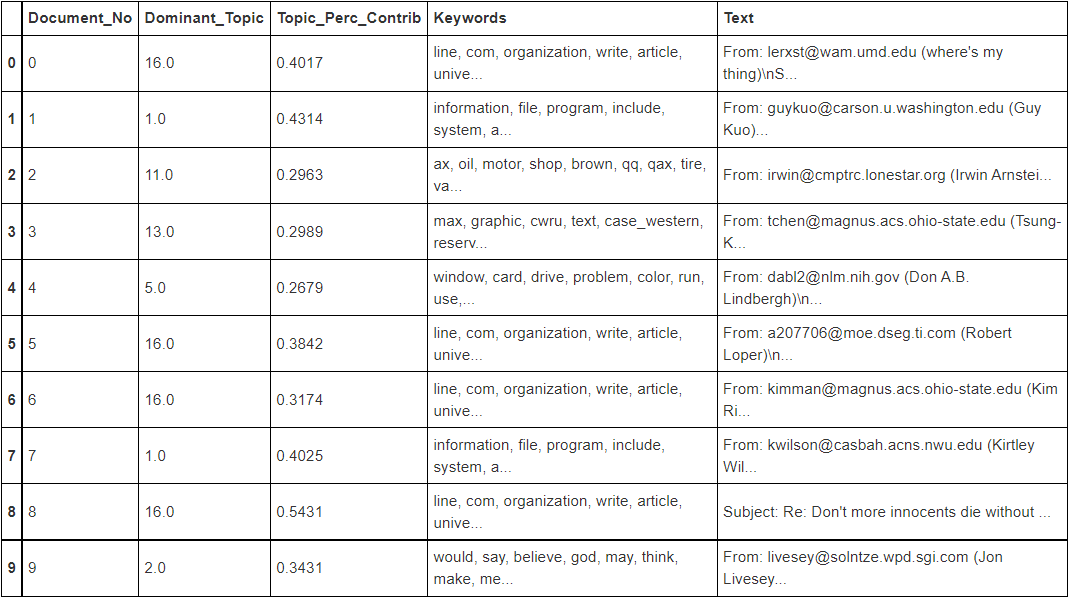
\includegraphics[width=1\textwidth]{
			mainTopics.png
		}
		\caption[Các topic chính của document sau khi được train bằng model LDA]{
			Các topic chính của document sau khi được train bằng model LDA  \label{mainTopics} \cite{WEBSITE:14}
		}
	\end{figure}
\end{enumerate}

\section{Kết luận}
Với bài toán Topic Modeling, việc xuất ra hết những từ/tài liệu quan trọng trong mỗi chủ đề không phải là điều tối ưu, đặc biệt với bộ dữ liệu lớn. Do vậy, giải pháp là ta chỉ hiển thị những từ/tài liệu thuộc top trong chủ đề. Điều này sẽ hữu ích nhất trong việc tìm được tên chủ đề. \cite{WEBSITE:15}
 
%\chapter{Các model nâng cao trong xử lý dữ liệu dạng văn bản}
\label{Chapter4}
\section{Tại sao cần các phương pháp này ?}

Các phương pháp trích xuất đặc trưng truyền thống (dựa trên số lượng) cho dữ liệu văn bản liên quan đến họ phương pháp rất phổ biến là Bag of Words hay bao gồm cả tần số như TF-IDF, N-gram... 

Mặc dù chúng đều là các phương pháp hiệu quả để trích xuất đặc trưng từ văn bản, nhưng do bản chất vốn có của các mô hình đó chỉ là xét trên các từ không có cấu trúc, như vậy chúng ta sẽ mất các thông tin bổ sung như ngữ nghĩa, cấu trúc, trình tự và ngữ cảnh xung quanh các từ gần đó mỗi tài liệu văn bản

Các mô hình nâng cao này có thể trích xuất được các thông tin sâu hơn có thể bao quát được cho cả các từ, thường được gọi là word embeddings.

\section{Mô hình Word2Vec}
Mô hình này được Google rạo ra vào năm 2013 và là mô hình sử dụng deep learning để tính toán và tạo ra các vectơ biểu diễn các từ và bao gồm được cả các tương đồng về ngữ cảnh và ngữ nghĩa của từ đó.

Về cơ bản, đây là mô hình học không giám sát, có thể áp dụng được cho những tập văn bản lớn, tạo ra vốn từ vựng và tạo ra embedding trong không gian vecto cho mỗi từ vựng đó.

Thông thường kích thước của vectơ embeddings và tổng số vectơ là kích thước của không gian từ vựng. Điều này làm cho số chiều của không gian vectơ này thấp hơn rất nhiều so với không gian vectơ được tạo ra bởi mô hình \textbf{Bag of Words} truyền thống.

Có hai kiến trúc khác nhau có thể sử dụng để tạo ra các vectơ embedding này bao gồm \cite{WEBSITE:17} \cite{WEBSITE:18}:
\begin{itemize}
	\item Mô hình \textbf{Continous Bag of Words (CBOW)}
	\item Mô hình \textbf{Skip-gram}
\end{itemize} 


\section{Mô hình Continuous Bag of Words (CBOW)}

Mô hình CBOW sẽ cố gắng dự đoán từ trung tâm (center word hoặc target word) dựa trên ngữ cảnh được tạo ra từ các từ xung quanh nó (surrounding words)

Chúng ta hãy xem xét một câu đơn giản \textbf{"the quick brown fox jumps over the lazy dog"}, chúng ta có thể có các cặp \textbf{ (context-window, target-word)} nếu chọn \textbf{context-window = 2} ta sẽ có \textbf{ ([quick, fox], brown), ([the, brown], quick), ([the, dog], lazy)}. Như vậy ta có thể dự đoán \textbf{target-word} dựa trên \textbf{context-window} như sau \ref{CBOW} \cite{WEBSITE:19}.


\begin{figure}[h!]
	\centering
	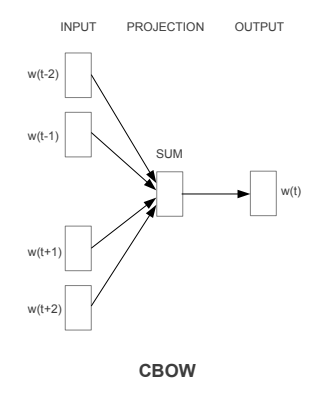
\includegraphics[width=0.8\textwidth]{
		CBOW.png
	}
	\caption[Mô hình CBOW]{
		Mô hình CBOW \label{CBOW}
	}
\end{figure}

\section{Xây dựng mô hình Continuous Bag of Words (CBOW)}

\textbf{ Việc xây dựng mô hình sẽ tập trung vào bốn bước sau}:
\begin{enumerate}
	\item \textbf{Xây dựng tập từ vựng}
	\item \textbf{Xây dựng CBOW generator (bao gồm các cặp [context-window, target-word])}
	\item \textbf{Xây dựng kiến trúc mô hình CBOW}
	\item \textbf{Huấn luyện mô hình}
	\item \textbf{Thu được embedding của các từ}			
\end{enumerate}

\subsection{Xây dựng tập từ vựng}
\lstinputlisting[style=codePython]{"Code/buildVocab.py"}
\textbf{Kết quả}:
\lstinputlisting[style=plaintext]{"Code/vocab.txt"}

\subsection{Xây dựng CBOW generator (bao gồm các cặp [context-window, target-word]}
\lstinputlisting[style=codePython]{"Code/buildCBOWgenerator.py"}
\textbf{Kết quả}:
\lstinputlisting[style=plaintext]{"Code/pairGenerator.txt"}

\subsection{Xây dựng kiến trúc mô hình CBOW}
\lstinputlisting[style=codePython]{"Code/buildCBOWDeep.py"}

\subsection{Huấn luyện mô hình}
\lstinputlisting[style=codePython]{"Code/TrainCBOW.py"}
\textbf{Kết quả}:
\lstinputlisting[style=plaintext]{"Code/CBOWRes.txt"}

\subsection{Thu về Embedding Words}
\lstinputlisting[style=codePython]{"Code/getWordsEmbeddings.py"}
\textbf{Kết quả}: \ref{CBOWRes}
\begin{figure}[h!]
	\centering
	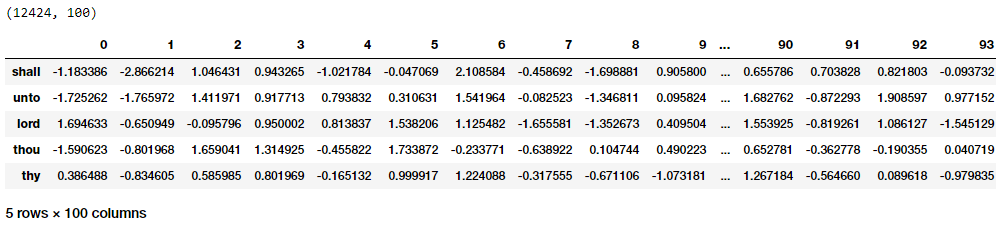
\includegraphics[width=1\textwidth]{
		CBOWRes.png
	}
	\caption[Embedding Words]{
		Embedding Words \label{CBOWRes}
	}
\end{figure}



 


%----------------------------------------------------------------------------------------
%	Phần 15: PHỤ LỤC (THESIS CONTENT - APPENDICES)
%----------------------------------------------------------------------------------------

\appendix % Nói với LaTeX rằng những chương về sau được tính là phụ lục

% Hãy thêm những phụ lục (appendix) của khóa luận/tiểu luận vào thư mục Appendices
% Hãy bỏ chú thích những dòng nếu bạn đã bổ sung những phụ lục vào

% Phụ lục A

\chapter{Các câu hỏi thường gặp} % Tên của phụ lục

\label{AppendixA} % Để trích dẫn chương này ở chỗ nào đó trong bài, hãy sử dụng lệnh \ref{AppendixA} 

%----------------------------------------------------------------------------------------

\section{Làm sao để thay đổi màu của đường dẫn liên kết?}

Màu sắc của đường dẫn có thể được thay đổi bằng các lệnh sau:

{\small\verb!\hypersetup{urlcolor=red}!}, hoặc

{\small\verb!\hypersetup{citecolor=green}!}, hoặc

{\small\verb!\hypersetup{allcolor=blue}!}.

\noindent Nếu bạn muốn ẩn toàn bộ đường dẫn, bạn có thể dùng lệnh:

{\small\verb!\hypersetup{allcolors=.}!}, hoặc thậm chí tốt hơn: 

{\small\verb!\hypersetup{hidelinks}!}.

\noindent Nếu bạn muốn hiển thị đường dẫn có màu trên file PDF còn ở bản in ra thì không, hãy sử dụng:

{\small\verb!\hypersetup{colorlinks=false}!}.


%----------------------------------------------------------------------------------------

\section{Làm sao để biểu diễn một bảng số liệu dài (hơn 1 trang), hoặc một bảng quá to?}

Thay vì sử dụng lệnh {\small\verb!\begin{table}!}, bạn hãy sử dụng lệnh {\small\verb!\begin{longtable}!}. Gói bổ trợ \code{longtable} (đã có sẵn trong template này) sẽ tự động giúp bạn ngắt bảng tại một vị trí khi bảng đã quá dài và biểu diễn phần còn lại của bảng ở những trang tiếp theo. Tài liệu về \code{longtable} bạn có thể tham khảo tại \href{https://mirror.kku.ac.th/CTAN/macros/latex/required/tools/longtable.pdf}{đường dẫn này}.

Trong trường hợp bảng số liệu dài theo bề ngang, bạn có thể xem xét phương án biểu diễn bảng số liệu theo chiều ngang của trang giấy như ví dụ Bảng~\ref{tab:treatments2} dưới đây. Để thực hiện cách này, bạn khai báo bảng như bình thường, rồi thay lệnh {\small\verb!\begin{table}!} bằng lệnh {\small\verb!\begin{sidewaystable}!}. Gói bổ trợ cho lệnh này đã có sẵn trong template này.

\begin{sidewaystable}
	\caption{Ảnh hưởng của phương pháp điều trị X và Y đối với bốn nhóm được nghiên cứu.}
	\label{tab:treatments2}
	\centering
	\begin{tabular}{l l l}
		\toprule
		\tabhead{Nhóm} & \tabhead{Phương pháp X} & \tabhead{Phương pháp Y} \\
		\midrule
		1	& 0.20	& 0.80	\\
		2	& 0.17	& 0.70	\\
		3	& 0.24	& 0.75	\\
		4	& 0.68	& 0.30	\\
		\bottomrule	\\
	\end{tabular}
\end{sidewaystable}


%----------------------------------------------------------------------------------------

\section{Làm sao để tìm đoạn code dưới định dạng bibtex cho tài liệu trích dẫn một cách hiệu quả?}

Bạn có thể tham khảo một số cách sau đây:

\begin{itemize}
	\item Cách 1: Sử dụng trang \href{https://scholar.google.com}{scholar.google.com}\\
	Bạn sẽ cần đi đến trang \href{https://scholar.google.com}{scholar.google.com} và hãy dán chính xác tên bài báo bạn muốn tìm kiếm. Sau đó bạn sẽ thấy một danh sách rất nhiều các đường dẫn đến bài báo và cả các bài báo tương tự mà bạn tìm kiếm. Hãy click vào biểu tượng: \textcolor{blue}{\faQuoteRight\;Cite}, rồi chọn tùy chọn \option{BibTeX} và bạn sẽ thấy đoạn code bạn cần.
	\item Cách 2: Sử dụng trang \href{https://www.researchgate.net/search}{researchgate.net}\\
	Bạn sẽ cần đi đến trang \href{https://www.researchgate.net/search}{researchgate.net} và hãy dán chính xác tên bài báo bạn muốn tìm kiếm. Sau đó bạn sẽ thấy một danh sách rất nhiều các đường dẫn đến bài báo và cả các bài báo tương tự mà bạn tìm kiếm. Hãy click vào tên bài báo phù hợp, sau đó click vào \option{Download citation}, rồi chọn tùy chọn \option{BibTeX} và \option{Citation only}. Để thuận tiện, bạn không cần download file chứa nội dung BibTeX về mà chỉ đơn giản chọn \option{Copy to clipboard} rồi dán nội dung vừa copy vào file \file{main.bib} của mình.
	\item Cách 3: Nếu một số tài liệu không xuất hiện ở cả hai trang phía trên, những tài liệu này thường là phần mềm hoặc kỉ yếu hoặc sách. Đối với phần mềm hoặc kỉ yếu, bạn có thể đi đến trang web chính thức chứa phần mềm hoặc kỉ yếu đó, nhiều khả năng là trang web sẽ hỗ trợ bạn trong việc trích dẫn. Đối với sách, bạn có nên tự xây dựng đoạn code BibTeX dựa trên một số đoạn code tương tự rồi thay đổi nội dung như số chương, số trang bạn đang muốn trích dẫn tới sao cho phù hợp.
\end{itemize}







% Phụ lục B

\chapter{Liệt kê source code} % Tên của phụ lục

\label{AppendixB} % Để trích dẫn chương này ở chỗ nào đó trong bài, hãy sử dụng lệnh \ref{AppendixB} 

%----------------------------------------------------------------------------------------

%\section{Ví dụ liệt kê code ngôn ngữ C/C++}
%
%Code tính khoảng thời gian giữa hai thời điểm cho trước. Lệnh thực hiện là:
%\begin{Verbatim}
%\lstinputlisting{"Code/TimeDiff.cpp"}
%\end{Verbatim}
%
%File \file{TimeDiff.cpp}:
%%https://www.programiz.com/cpp-programming/examples/time-structure
%\lstinputlisting{"Code/TimeDiff.cpp"}


%----------------------------------------------------------------------------------------

%\section{Ví dụ liệt kê thông tin ở terminal (console/command prompt) từ file text}
%
%Sau khi biên dịch và chạy file \file{TimeDiff.cpp}, kết quả chạy được hiển thị ở terminal. Trong trường hợp bạn muốn liệt kê quá trình chạy, bạn có thể copy đoạn text ở terminal vào một file text, và liệt kê chúng chẳng hạn như:
%\begin{Verbatim}
%\lstinputlisting[style=console]{"Code/TimeDiff.txt"}
%\end{Verbatim}
%
%File \file{TimeDiff.txt}:
%\lstinputlisting[style=console]{"Code/TimeDiff.txt"}


%----------------------------------------------------------------------------------------

\section{Thuật toán LSA}

\lstinputlisting[style=codePython]{"Code/LSA.py"}
\newpage

\section{Thuật toán LDA}

\lstinputlisting[style=codePython]{"Code/lda.py"}

\newpage
\section{Model CBOW}
\lstinputlisting[style=codePython]{"Code/CBOW.py"}
%----------------------------------------------------------------------------------------

%\section{Ví dụ liệt kê code ngôn ngữ Matlab}
%
%Code biểu diễn bản chất và sai số của phương pháp Euler và Heun trong việc giải phương trình vi phân. Lệnh thực hiện là:
%\begin{Verbatim}
%\lstinputlisting[style=codeMatlab]{"Code/EulerVisualization.m"}
%\end{Verbatim}
%
%File \file{EulerVisualization.m}:
%\lstinputlisting[style=codeMatlab]{"Code/EulerVisualization.m"}


%----------------------------------------------------------------------------------------

%\section{Ví dụ liệt kê file text thông thường (plain text)}
%
%Một file text lưu giữ thông số của một lần chạy mô phỏng động học phân tử. Lệnh thực hiện là:
%\begin{Verbatim}
%\lstinputlisting[style=plaintext]{"Code/minim.mdp"}
%\end{Verbatim}
%
%File \file{minim.mdp}:
%\lstinputlisting[style=plaintext]{"Code/minim.mdp"}




%\include{Appendices/AppendixC}


%----------------------------------------------------------------------------------------
%	(KHÔNG CHỈNH SỬA PHẦN NÀY)
%
%	Phần 16: TÀI LIỆU THAM KHẢO
%----------------------------------------------------------------------------------------

\begin{spacing}{1.15}
	\printbibliography[heading=bibintoc, title=Tài liệu tham khảo] % In ra tài liệu tham khảo
\end{spacing}

%----------------------------------------------------------------------------------------

\end{document}  
